% Options for packages loaded elsewhere
\PassOptionsToPackage{unicode}{hyperref}
\PassOptionsToPackage{hyphens}{url}
\PassOptionsToPackage{dvipsnames,svgnames,x11names}{xcolor}
%
\documentclass[
]{article}

\usepackage{amsmath,amssymb}
\usepackage{iftex}
\ifPDFTeX
  \usepackage[T1]{fontenc}
  \usepackage[utf8]{inputenc}
  \usepackage{textcomp} % provide euro and other symbols
\else % if luatex or xetex
  \usepackage{unicode-math}
  \defaultfontfeatures{Scale=MatchLowercase}
  \defaultfontfeatures[\rmfamily]{Ligatures=TeX,Scale=1}
\fi
\usepackage{lmodern}
\ifPDFTeX\else  
    % xetex/luatex font selection
\fi
% Use upquote if available, for straight quotes in verbatim environments
\IfFileExists{upquote.sty}{\usepackage{upquote}}{}
\IfFileExists{microtype.sty}{% use microtype if available
  \usepackage[]{microtype}
  \UseMicrotypeSet[protrusion]{basicmath} % disable protrusion for tt fonts
}{}
\makeatletter
\@ifundefined{KOMAClassName}{% if non-KOMA class
  \IfFileExists{parskip.sty}{%
    \usepackage{parskip}
  }{% else
    \setlength{\parindent}{0pt}
    \setlength{\parskip}{6pt plus 2pt minus 1pt}}
}{% if KOMA class
  \KOMAoptions{parskip=half}}
\makeatother
\usepackage{xcolor}
\setlength{\emergencystretch}{3em} % prevent overfull lines
\setcounter{secnumdepth}{-\maxdimen} % remove section numbering
% Make \paragraph and \subparagraph free-standing
\makeatletter
\ifx\paragraph\undefined\else
  \let\oldparagraph\paragraph
  \renewcommand{\paragraph}{
    \@ifstar
      \xxxParagraphStar
      \xxxParagraphNoStar
  }
  \newcommand{\xxxParagraphStar}[1]{\oldparagraph*{#1}\mbox{}}
  \newcommand{\xxxParagraphNoStar}[1]{\oldparagraph{#1}\mbox{}}
\fi
\ifx\subparagraph\undefined\else
  \let\oldsubparagraph\subparagraph
  \renewcommand{\subparagraph}{
    \@ifstar
      \xxxSubParagraphStar
      \xxxSubParagraphNoStar
  }
  \newcommand{\xxxSubParagraphStar}[1]{\oldsubparagraph*{#1}\mbox{}}
  \newcommand{\xxxSubParagraphNoStar}[1]{\oldsubparagraph{#1}\mbox{}}
\fi
\makeatother


\providecommand{\tightlist}{%
  \setlength{\itemsep}{0pt}\setlength{\parskip}{0pt}}\usepackage{longtable,booktabs,array}
\usepackage{calc} % for calculating minipage widths
% Correct order of tables after \paragraph or \subparagraph
\usepackage{etoolbox}
\makeatletter
\patchcmd\longtable{\par}{\if@noskipsec\mbox{}\fi\par}{}{}
\makeatother
% Allow footnotes in longtable head/foot
\IfFileExists{footnotehyper.sty}{\usepackage{footnotehyper}}{\usepackage{footnote}}
\makesavenoteenv{longtable}
\usepackage{graphicx}
\makeatletter
\def\maxwidth{\ifdim\Gin@nat@width>\linewidth\linewidth\else\Gin@nat@width\fi}
\def\maxheight{\ifdim\Gin@nat@height>\textheight\textheight\else\Gin@nat@height\fi}
\makeatother
% Scale images if necessary, so that they will not overflow the page
% margins by default, and it is still possible to overwrite the defaults
% using explicit options in \includegraphics[width, height, ...]{}
\setkeys{Gin}{width=\maxwidth,height=\maxheight,keepaspectratio}
% Set default figure placement to htbp
\makeatletter
\def\fps@figure{htbp}
\makeatother
% definitions for citeproc citations
\NewDocumentCommand\citeproctext{}{}
\NewDocumentCommand\citeproc{mm}{%
  \begingroup\def\citeproctext{#2}\cite{#1}\endgroup}
\makeatletter
 % allow citations to break across lines
 \let\@cite@ofmt\@firstofone
 % avoid brackets around text for \cite:
 \def\@biblabel#1{}
 \def\@cite#1#2{{#1\if@tempswa , #2\fi}}
\makeatother
\newlength{\cslhangindent}
\setlength{\cslhangindent}{1.5em}
\newlength{\csllabelwidth}
\setlength{\csllabelwidth}{3em}
\newenvironment{CSLReferences}[2] % #1 hanging-indent, #2 entry-spacing
 {\begin{list}{}{%
  \setlength{\itemindent}{0pt}
  \setlength{\leftmargin}{0pt}
  \setlength{\parsep}{0pt}
  % turn on hanging indent if param 1 is 1
  \ifodd #1
   \setlength{\leftmargin}{\cslhangindent}
   \setlength{\itemindent}{-1\cslhangindent}
  \fi
  % set entry spacing
  \setlength{\itemsep}{#2\baselineskip}}}
 {\end{list}}
\usepackage{calc}
\newcommand{\CSLBlock}[1]{\hfill\break\parbox[t]{\linewidth}{\strut\ignorespaces#1\strut}}
\newcommand{\CSLLeftMargin}[1]{\parbox[t]{\csllabelwidth}{\strut#1\strut}}
\newcommand{\CSLRightInline}[1]{\parbox[t]{\linewidth - \csllabelwidth}{\strut#1\strut}}
\newcommand{\CSLIndent}[1]{\hspace{\cslhangindent}#1}

\usepackage{booktabs}
\usepackage{caption}
\usepackage{longtable}
\usepackage{colortbl}
\usepackage{array}
\makeatletter
\@ifpackageloaded{caption}{}{\usepackage{caption}}
\AtBeginDocument{%
\ifdefined\contentsname
  \renewcommand*\contentsname{Table of contents}
\else
  \newcommand\contentsname{Table of contents}
\fi
\ifdefined\listfigurename
  \renewcommand*\listfigurename{List of Figures}
\else
  \newcommand\listfigurename{List of Figures}
\fi
\ifdefined\listtablename
  \renewcommand*\listtablename{List of Tables}
\else
  \newcommand\listtablename{List of Tables}
\fi
\ifdefined\figurename
  \renewcommand*\figurename{Figure}
\else
  \newcommand\figurename{Figure}
\fi
\ifdefined\tablename
  \renewcommand*\tablename{Table}
\else
  \newcommand\tablename{Table}
\fi
}
\@ifpackageloaded{float}{}{\usepackage{float}}
\floatstyle{ruled}
\@ifundefined{c@chapter}{\newfloat{codelisting}{h}{lop}}{\newfloat{codelisting}{h}{lop}[chapter]}
\floatname{codelisting}{Listing}
\newcommand*\listoflistings{\listof{codelisting}{List of Listings}}
\makeatother
\makeatletter
\makeatother
\makeatletter
\@ifpackageloaded{caption}{}{\usepackage{caption}}
\@ifpackageloaded{subcaption}{}{\usepackage{subcaption}}
\makeatother
\makeatletter
\@ifpackageloaded{sidenotes}{}{\usepackage{sidenotes}}
\@ifpackageloaded{marginnote}{}{\usepackage{marginnote}}
\makeatother

\ifLuaTeX
  \usepackage{selnolig}  % disable illegal ligatures
\fi
\usepackage{bookmark}

\IfFileExists{xurl.sty}{\usepackage{xurl}}{} % add URL line breaks if available
\urlstyle{same} % disable monospaced font for URLs
\hypersetup{
  pdftitle={Twenty years of dynamic occupancy models: a review of applications and a look towards the future},
  colorlinks=true,
  linkcolor={blue},
  filecolor={Maroon},
  citecolor={Blue},
  urlcolor={Blue},
  pdfcreator={LaTeX via pandoc}}


\title{Twenty years of dynamic occupancy models: a review of
applications and a look towards the future}
\author{Saoirse Kelleher \and Natalie Briscoe \and Gurutzeta
Guillera-Arroita \and Jane Elith}
\date{2024-09-10}

\begin{document}
\maketitle
\begin{abstract}
Describing patterns of species occupancy across landscapes and
throughout time is a key objective of much ecological research.
Nonetheless, reliably estimating occupancy can be a challenge,
particularly when common issues such as imperfect detection and shifting
distributions are at play. The dynamic, multi-season occupancy model
(DOM) offers a framework for occupancy estimation which explicitly
accounts for observation error, while also incorporating additional
mechanistic process by explicitly estimating colonisation and extinction
rates. In the two decades since its introduction, the DOM has become a
popular tool for describing patterns in occupancy, exploring the
environmental drivers of species occurence, and, more recently, for
predicting species occupancy to new locations and to future conditions.

In this review we examine how ecologists have applied the DOM in its
first two decades of use. Based on a sample of articles fitting DOMs to
field ecological data, we explore the systems in which these models have
been used, how data were collected for them, and how authors have built
their models to achieve their objectives. Our findings indicate that the
DOM is an particularly flexible tool readily applied to a range of
diverse taxa from around the globe, capable of being used to estimate
occupancy at study sites ranging from local to continental scales over
time periods from months to decades. The DOM framework is also amenable
to extension, further broadening their utility to address a wide range
of ecological questions.

A key aim of this review is to explore how users of DOMs have
incorporated covariates into their models to describe variation in
occupancy through space and time. Broadly speaking, model complexity in
DOMs tends to be low, with relatively few covariates considered for
inclusion and most relationships represented as simple linear terms.
Considerable variation also exists in the procedures used for covariate
selection, and limited research has been conducted on how these choices
may influence model performance and inference. Furthermore, only a
fraction of articles appear to evaluate models (either by
goodness-of-fit testing or prediction validation). Likewise, little
guidance exists on how to approach this task in DOMs. These
uncertainties in the modelling process should be key priorities for
future research on DOMs given their increasing use in applied ecological
research.
\end{abstract}


\section{Introduction}\label{introduction}

The description of patterns of species occupancy across landscapes has
been a long-standing subject of ecological research (Humboldt, 1849). An
understanding of where a species exists, which factors lead to its
presence, and how its distribution may be changing can be applied in
many ways. Descriptions of how widespread a species is and where it
occurs are the foundation of monitoring programs and important for
assessing conservation status, while identifying potential drivers of
occurrence can help inform potential management actions. Robust
knowledge of the occupancy patterns of a species also helps us to
predict where a species is most likely to occur, both under present
conditions and in hypothetical future scenarios.

While occupancy is a useful concept, it is also a challenging quantity
to describe, measure, and estimate. The need to understand and describe
species occupancy has led to the development of several popular
modelling approaches, including stochastic patch occupancy models
(Gutiérrez-Arellano et al., 2024) commonly used to study meta-population
dynamics, and species distribution models (SDMs, Franklin, 2010) widely
used to explore species occurrence at larger scales. However, several
factors can make occupancy a difficult quantity to estimate. For
instance, simple presence/absence data of species observations can be
biased when species are detected imperfectly, as is the case with most
wildlife field data. Generally speaking, it is impossible to determine
whether a location is truly unoccupied or whether the species occurs but
was not detected by the observer (Gu \& Swihart, 2004; Lahoz-Monfort et
al., 2014). Despite the ubiquity of imperfect detection in data
collection, many models fit to presence/absence data make no adjustment
for this source of bias (Kellner \& Swihart, 2014). Another challenge
for modelling occupancy is the difficulty in describing populations
under non-equilibrium conditions, where a species occurrence pattern and
relationship to its environment is in flux (Dormann, 2007; Elith et al.,
2010). These conditions often occur during biological invasions and
climate change driven range shifts, both conservation priorities and
increasingly common scenarios in the Anthropocene (Bertelsmeier et al.,
2013; Lenoir \& Svenning, 2015).

The site occupancy models first introduced by MacKenzie et al. (2002)
set the foundation for a powerful framework for modelling
presence/absence data while accounting for each of these challenges
(Guillera-Arroita \& Lahoz-Monfort, 2017). Drawing on principles from
the mark-recapture literature, occupancy models use multiple resurveys
of sites to estimate detection probabilities and correct for bias in
estimates of site occupancy. Originally a static model, MacKenzie et al.
(2003) extended this model for use in multiple time-steps by explicitly
describing the process of changing occupancy via colonisation and
extinction, relaxing assumptions of equilibrium and allowing description
of patterns of site occupancy through time. This dynamic occupancy model
(DOM) balances complexity and feasibility, explicitly describing the key
processes which drive occupancy dynamics while requiring reasonably
simple-to-collect presence absence/data instead of the detailed
demographic or abundance data required by more process-explicit models
(Briscoe et al., 2019). These features make the DOM an important tool,
with uses for tasks including hypothesis testing of relationships
between occupancy and the environment, explorations of the key drivers
of occupancy, and even prediction of occupancy under future conditions
(Briscoe et al., 2021; Kéry et al., 2013).

In this review we examine how dynamic occupancy models have been used by
ecologists in the two decades since their inception. Following an
introduction to the model's form and assumptions, we present the results
of a systematic review exploring how researchers have applied the DOM to
ecological data, with emphasis on how they collected their data,
selected covariates, and evaluated their models. Based on these results
we highlight the DOM's flexibility as a tool for understanding species
occurrence, examine approaches to the model building process, and
outline key priorities for future research involving this model class.

\subsubsection{Dynamic occupancy model form and
assumptions}\label{dynamic-occupancy-model-form-and-assumptions}

The DOM structure encompasses two processes: the ecological process of
site occupancy dynamics describing the presence or absence of a species
at a site at any point in time, and the observational process of
detection describing whether a species is observed at a site where it is
present (Figure~\ref{fig-modelform}). Sites exist in either an occupied
or unoccupied state. In the first time step, occupancy state at each
site is determined by the probability of initial occupancy. In following
time steps, occupancy state can change according to a Markovian process
where occupancy is predicated on the site's state in the prior time-step
and the probabilities of colonisation and local extinction. In the
observation component of the DOM, the model explicitly accounts for
imperfect detection. At occupied sites, the detection probability
describes whether or not the species is observed during a survey; under
the DOM's original parameterisation, it is assumed that false-positive
detections at unoccupied sites never occur.

\begin{figure}

\centering{

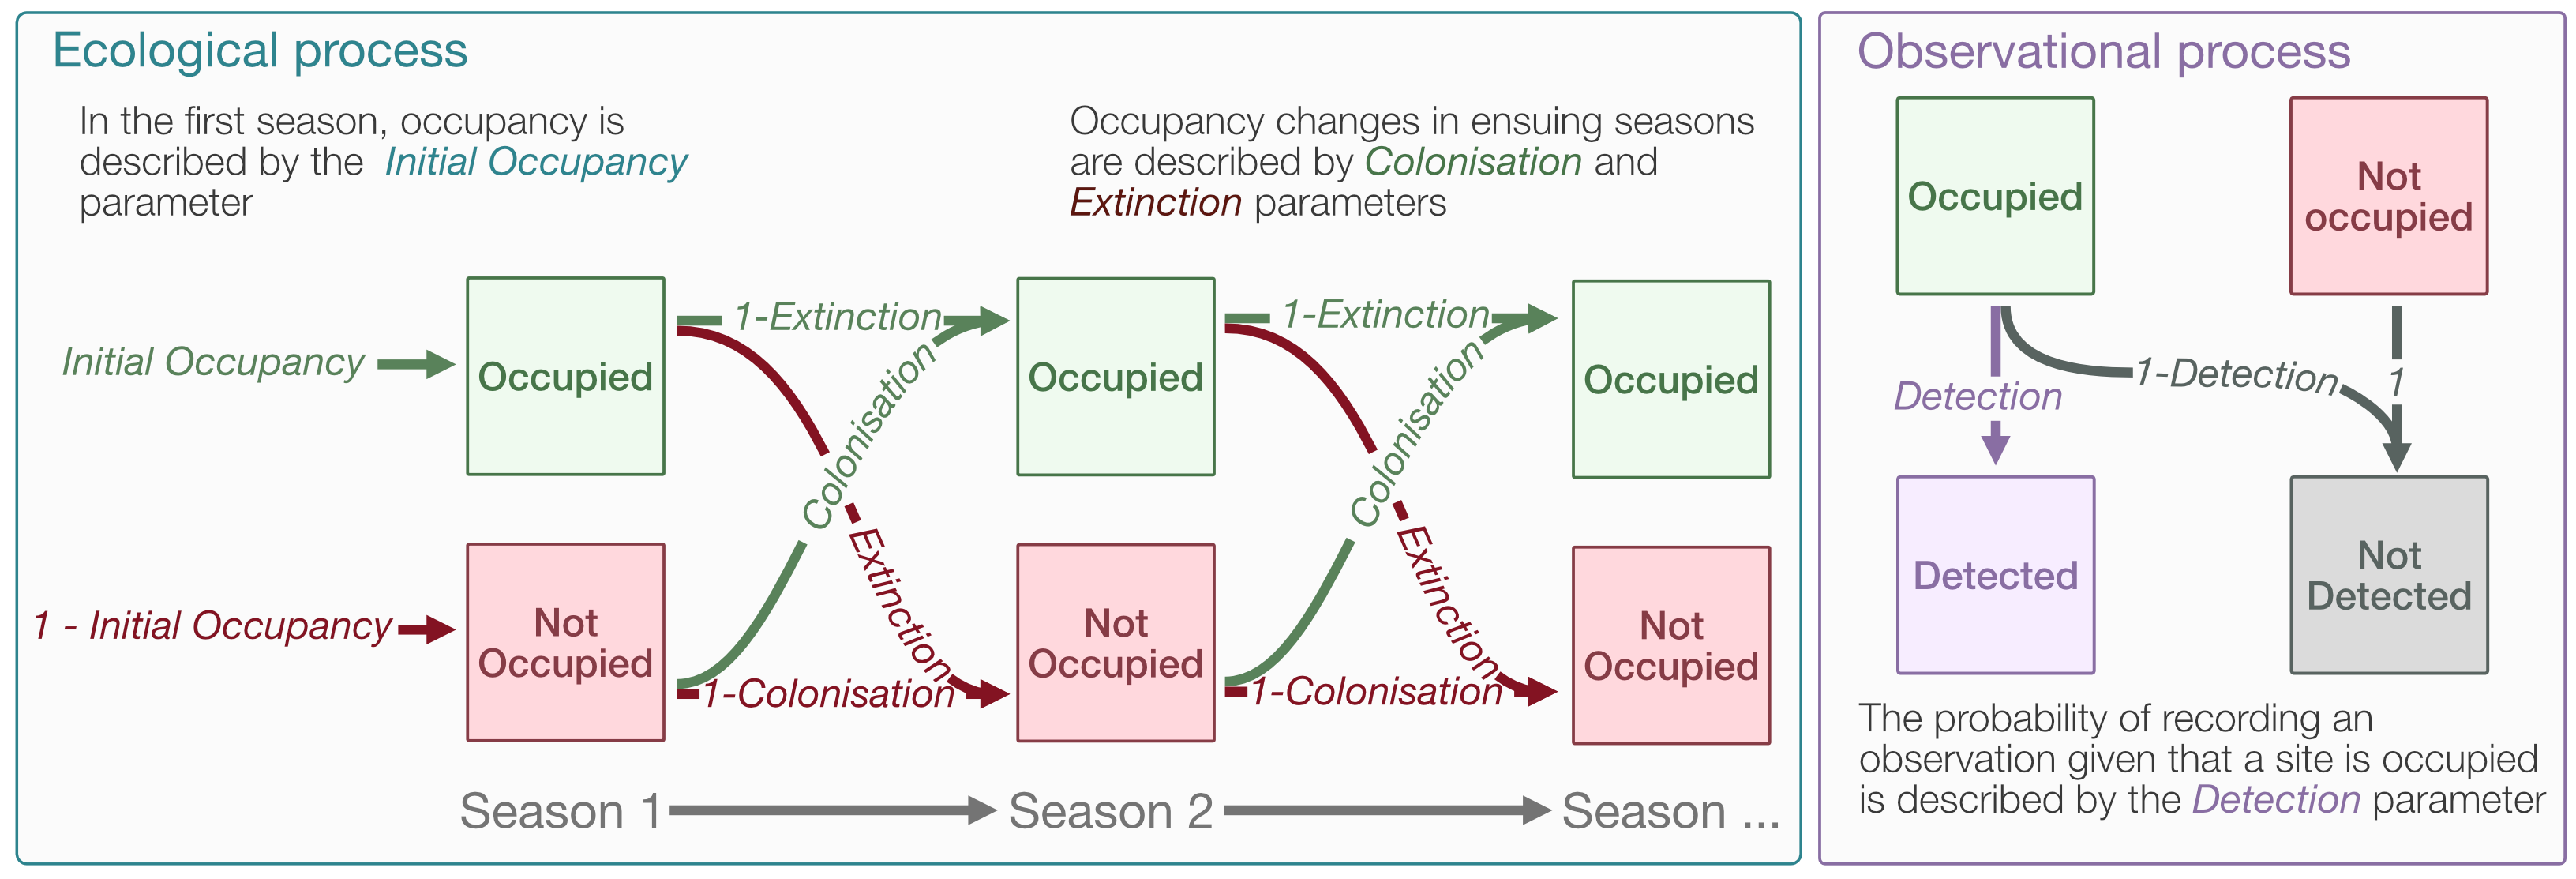
\includegraphics{Figures/ModelForm.png}

}

\caption{\label{fig-modelform}The form of the dynamic occupancy model as
described by MacKenzie et al. (2003). The ecological process submodel
describes changes in occupancy over time, where occupancy in the first
season is given by the probability of initial occupancy and occupancy in
ensuing seasons is governed by colonisation and extinction
probabilities. The observational process submodel describes
detectability, where the probability of detecting a species given that a
site is occupied is given by the detection probability. At sites which
are truly unoccupied, it is assumed that the species is never detected
(i.e., no false positives).}

\end{figure}%

To disentangle the ecological and observational processes the DOM
requires a hierarchical sampling design as depicted in
Figure~\ref{fig-surveys}. Under this design, observations at a site
occur during distinct, time-bound seasons within which it is assumed
site occupancy does not change (that is, sites are closed to changes in
occupancy). In each season multiple observations are conducted,
permitting estimation of the probability of detection conditional on
occupancy. Most frequently these repeat observations are collected by
revisiting the site on separate occasions, although they can also be
attained by alternative means: examples include conducting surveys at
multiple locations within a site, using multiple observers during a
survey, or recording the time elapsed until a detection is recorded
(Guillera-Arroita \& Lahoz-Monfort, 2017). It is important to note that
it is not necessary for the same number of observations to occur in each
year or for each site, and that the DOM accommodates for missing data;
this allows for considerably greater flexibility in data inputs.

\begin{figure}

\centering{

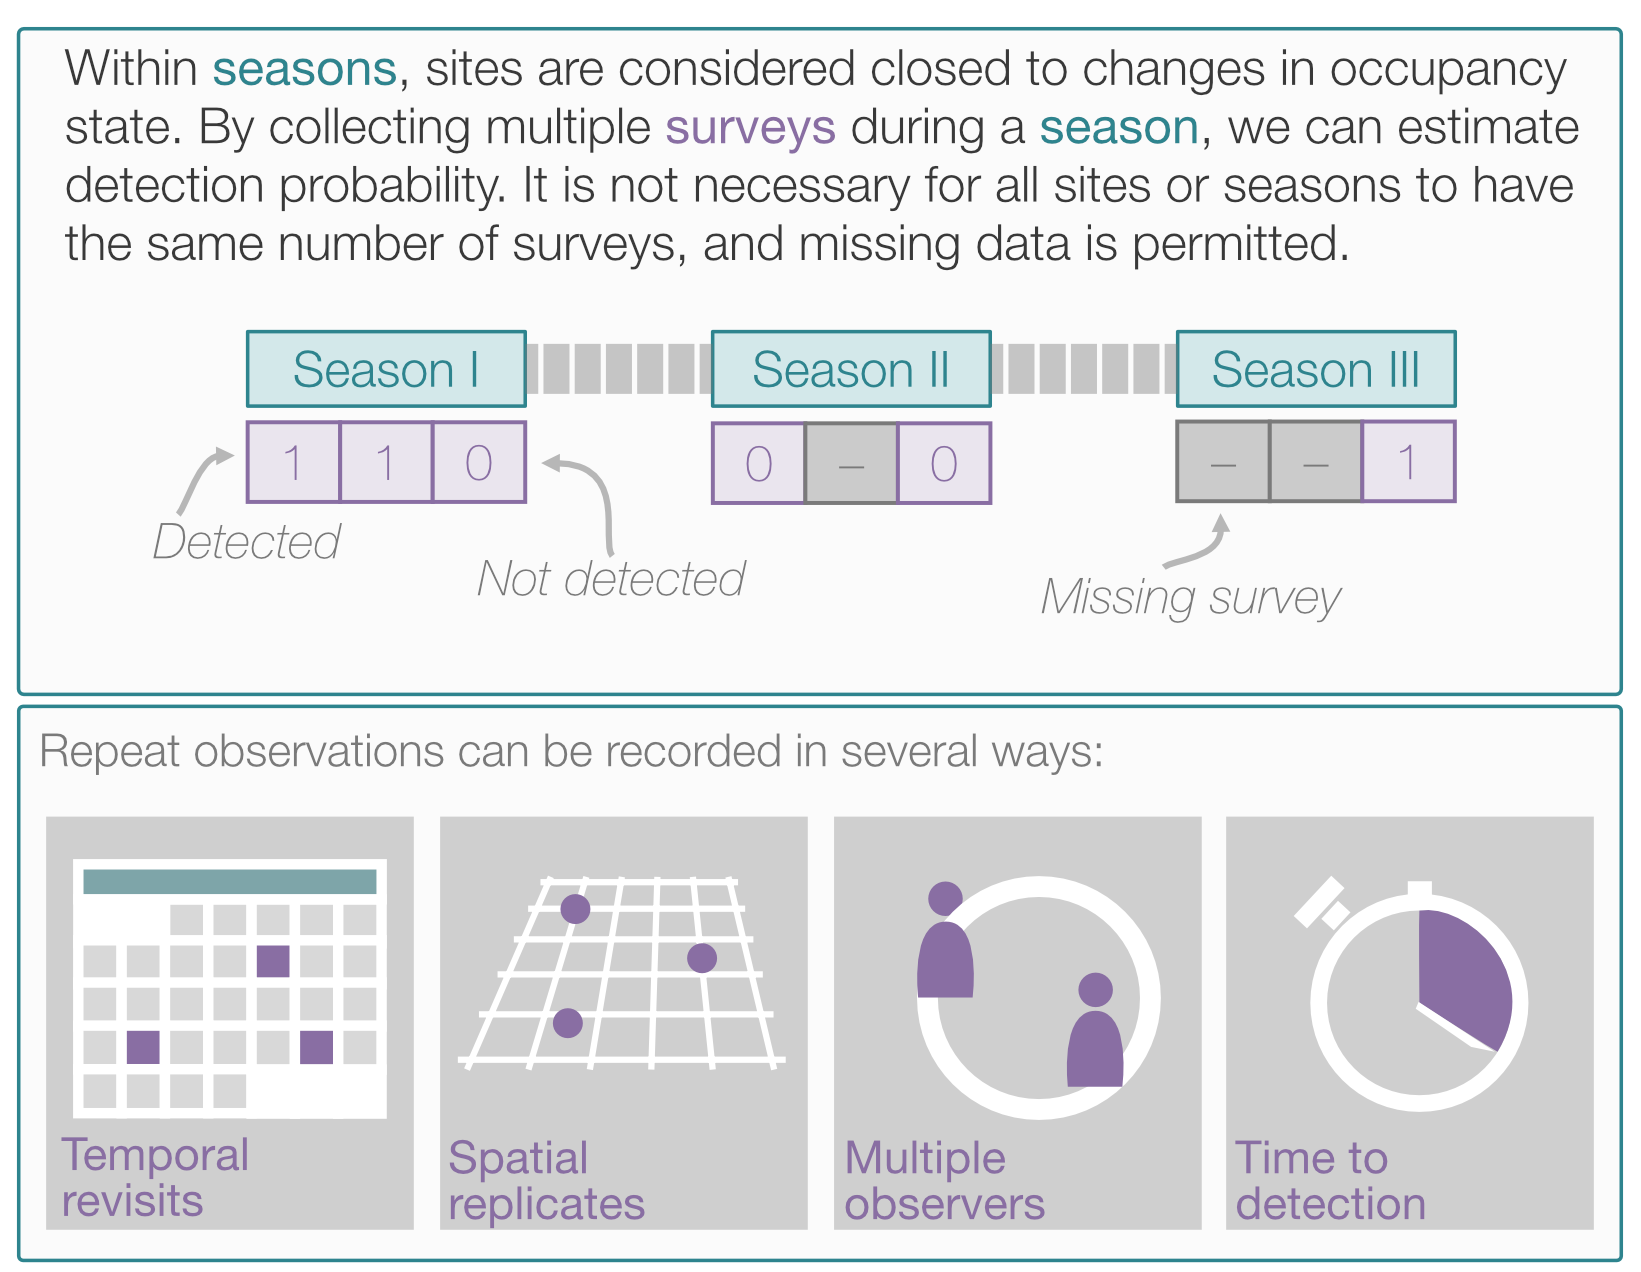
\includegraphics{Figures/SurveyDesign.png}

}

\caption{\label{fig-surveys}The sampling design of the standard dynamic
occupancy model. During seasons, also called primary occasions, sites
are considered closed to changes in true occupancy state; occupancy
state may only change between seasons. Within each season, multiple
observations (`secondary occasions') are conducted to record the
observed presence or absence of the species at each site. These multiple
observations may be recorded in many ways: sites can be revisited
multiple times within a season, surveys can be conducted at multiple
points within a larger site, multiple observers can conduct surveys
contemporaneously, or the time elapsed prior to a detection occurring
can be recorded. Note that it is not necessary for each site or season
to have the same number of observations, and that missing data can be
accommodated.}

\end{figure}%

DOMs make a number of key assumptions requiring careful consideration by
model users, which we outline here as our review interrogates related
aspects of model building.

\begin{enumerate}
\def\labelenumi{\Roman{enumi}.}
\item
  \textbf{False positive detections do not occur}. While this assumption
  can be safely met in many studies, it is not necessarily guaranteed
  when working with more cryptic species or less reliable survey
  methods. McClintock et al. (2010) and D. A. W. Miller et al. (2015)
  comment on the bias induced when false positives occur and are not
  accounted for, highlighting the need for authors to consider how
  certain their detections truly are. Significantly, even genuine
  detections of a species can be considered `false positives' when they
  do not represent the intended definition of occupancy, such as
  detections of transient individuals when the intent is to estimate
  breeding occupancy (Berigan et al., 2019). Where this assumption can
  not reasonably met, model extensions designed to account for false
  positive error should be considered.
\item
  \textbf{Sites are closed to occupancy between seasons.} This
  requirement, best known as the `closure assumption,' has also been
  subject to considerable discussion around the bias which is introduced
  when it is violated (Otto et al., 2013; Rota et al., 2009). Closure is
  dependent not only on the life history of the species, but also on the
  definition of occupancy used by researchers --- short seasons may
  represent dynamics more representative of species `use,' and Valente
  et al. (2017) discuss the difficultly in distinguishing between
  temporary emigration and local extinction. Model extensions to relax
  the closure assumption have been developed, including Kendall et al.
  (2013)'s approach using staggered arrival and departure periods
  between sites. A more pertinent approach for most studies, however, is
  careful consideration of ecologically relevant seasons corresponding
  to an appropriate definition of occupancy.
\item
  \textbf{Heterogeneity in occupancy and detection is accounted for.} As
  with any approach for modelling species occurrence, it is assumed that
  DOMs appropriately capture variation in occupancy patterns and species
  detectability across the study system. Generally, this is achieved by
  allowing model parameters to vary with respect to covariates
  representing the environmental factors which may be expected to
  influence these parameters. An important element of this assumption is
  that the likelihood of detection of a species depends not only on the
  observability of the species, but also on factors like habitat
  suitability which influence species abundance and activity
  (Guillera-Arroita \& Lahoz-Monfort, 2017). While no model will fully
  account for the complexity inherent in patterns of species occupancy
  and detection, failure to capture key drivers is likely to introduce
  bias and confound inference made from model estimates. Compared to the
  first two assumptions mentioned, this aspect of DOMs has been less
  thoroughly discussed and comparatively little is known about how this
  latent heterogeneity can influence model performance.
\end{enumerate}

Since its original description in MacKenzie et al. (2003), the DOM has
been further developed with numerous model extensions and alternative
formulations including implementations accounting for false positives
(D. Miller et al., 2011; D. A. W. Miller et al., 2015; Royle \& Link,
2006), multiple states beyond occupied and unoccupied (Nichols et al.,
2007), and jointly estimated multi-species models (Dorazio et al.,
2010). For a comprehensive discussion of the most common extensions and
their applications see Bailey et al. (2014) and Guillera-Arroita \&
Lahoz-Monfort (2017), as well as Devarajan et al. (2020) for a more
detailed review of multi-species occupancy models.

\section{Systematic review methods}\label{systematic-review-methods}

To assess how DOMs have been applied in the years since their
introduction we gathered a representative sample of articles fitting
them to field ecological data. A pool of candidate articles was
generated using two queries on Web of Science. The first of these
included all articles from 2004-2023 which cite MacKenzie et al. (2003).
To capture any additiona relevant articles which did not directly cite
MacKenzie et al. (2003), a second query was generated searching articles
in the same time-span matching the terms ``\emph{dynamic occupancy
model*}'', ``\emph{multi-season occupancy model*}'', or
``\emph{occupancy dynamic*}''; articles including each of
``\emph{occupancy}'', ``\emph{colonization}'',
``\emph{extinction/persistence}'', and ``\emph{detection}''; and
articles with the term ``\emph{occupancy}'' located near
``\emph{dynamic}'' in the title, key terms, or abstract. As we were
interested in how DOMs use has changed through time, we divided all
articles across four-year-long strata spanning 2004-2007, 2008-2011,
2012-2015, 2016-2019, and 2020-2024. From each of these strata we
randomly selected 20 articles for inclusion in the review. Articles
which did not meet inclusion criteria were replaced from within their
own strata.

As our review focuses only on applications of the dynamic multi-season
occupancy model of MacKenzie et al. (2003) and its extensions, we
included articles which fit a model meeting the following criteria: i)
uses non-simulated, field-collected, presence-absence data; ii) relies
on data from multiple sites which can exist in at least two states,
including an occupied and unoccupied state; iii) has multiple seasons,
between which sites may change states conditional on the prior season's
occupancy state and transition probabilities such as colonisation and
extinction; and iv) contains at least one parameter describing the
detection process.

For each article we recorded key details on authorship, research
objectives, study taxa and system, survey methods, and modelling
approach. To examine the reasons why authors used DOMs, we allocated
each article to one or more category of objective based on the study's
stated aims. The possible categories were \emph{Observing trends}, where
authors express interest in estimates of site occupancy, colonisation,
extinction, or detection probabilities; \emph{Testing relationships},
where authors explore specific predefined hypotheses of relationships
between covariates and model parameters; \emph{Identifying drivers},
where authors attempt to find which covariates influence model
parameters; \emph{Predicting temporally}, where authors predict site
occupancy under future conditions, \emph{Predicting spatially}, where
authors predict site occupancy to unsurveyed locations, and
\emph{Developing methods}, where authors introduce, test, or demonstrate
aspects of dynamic occupancy models.

We recorded details on the type of organisms (bird, mammal, etc.)
modelled in each article, and the means by which multiple species were
modelled where applicable. Taxa were denoted as threatened either when
they are listed on the IUCN Red List of Species or when authors indicate
that they are threatened. This deference to authors' representation of
conservation status was made to account for sub-species which lack
listings or species which are of more local concern. Study locality and
size was documented; the size of the study area being defined as the
intended area of inference which contained all sites --- this was
measured to the order of magnitude to account for uncertainty in
reporting.

We were particularly interested in how authors navigated the modelling
process, from covariate selection through model evaluation. To this end,
we recorded all covariates considered in each study regardless of
whether they were or were not included in final models. Key traits of
each covariate were recorded including their general category, whether
they were directly observed or remotely sensed, whether they were static
or varied between seasons, and how they were presented in the model (as
a linear term, a polynomial term, or as part of an interaction with
another covariate (James et al., 2021)). Model selection procedures were
also sorted into non-exclusive categories including \emph{A priori},
where only one model was considered; \emph{candidate suite}, where a
predefined set of models was considered; \emph{sequential,} where
covariates were selected parameter-by-parameter; and \emph{simple
precursors}, where selection was preceded by another simpler model
implementation. Finally, for each model we documented whether
goodness-of-fit was tested and reported, as well as whether model
performance was assessed by validation with either in or out-of-sample
data. For the full spreadsheet of data collected and further details on
categorisation, see supplementary material.

\section{Applications of dynamic occupancy
models}\label{applications-of-dynamic-occupancy-models}

A total of 92 articles were included for this review. Based on the
acceptance rates within each strata and quantity of unprocessed
articles, an estimated 496 of the 1152 unreviewed articles in our sample
would have met inclusion criteria (Figure~\ref{fig-coverage}).

\begin{figure}

\centering{

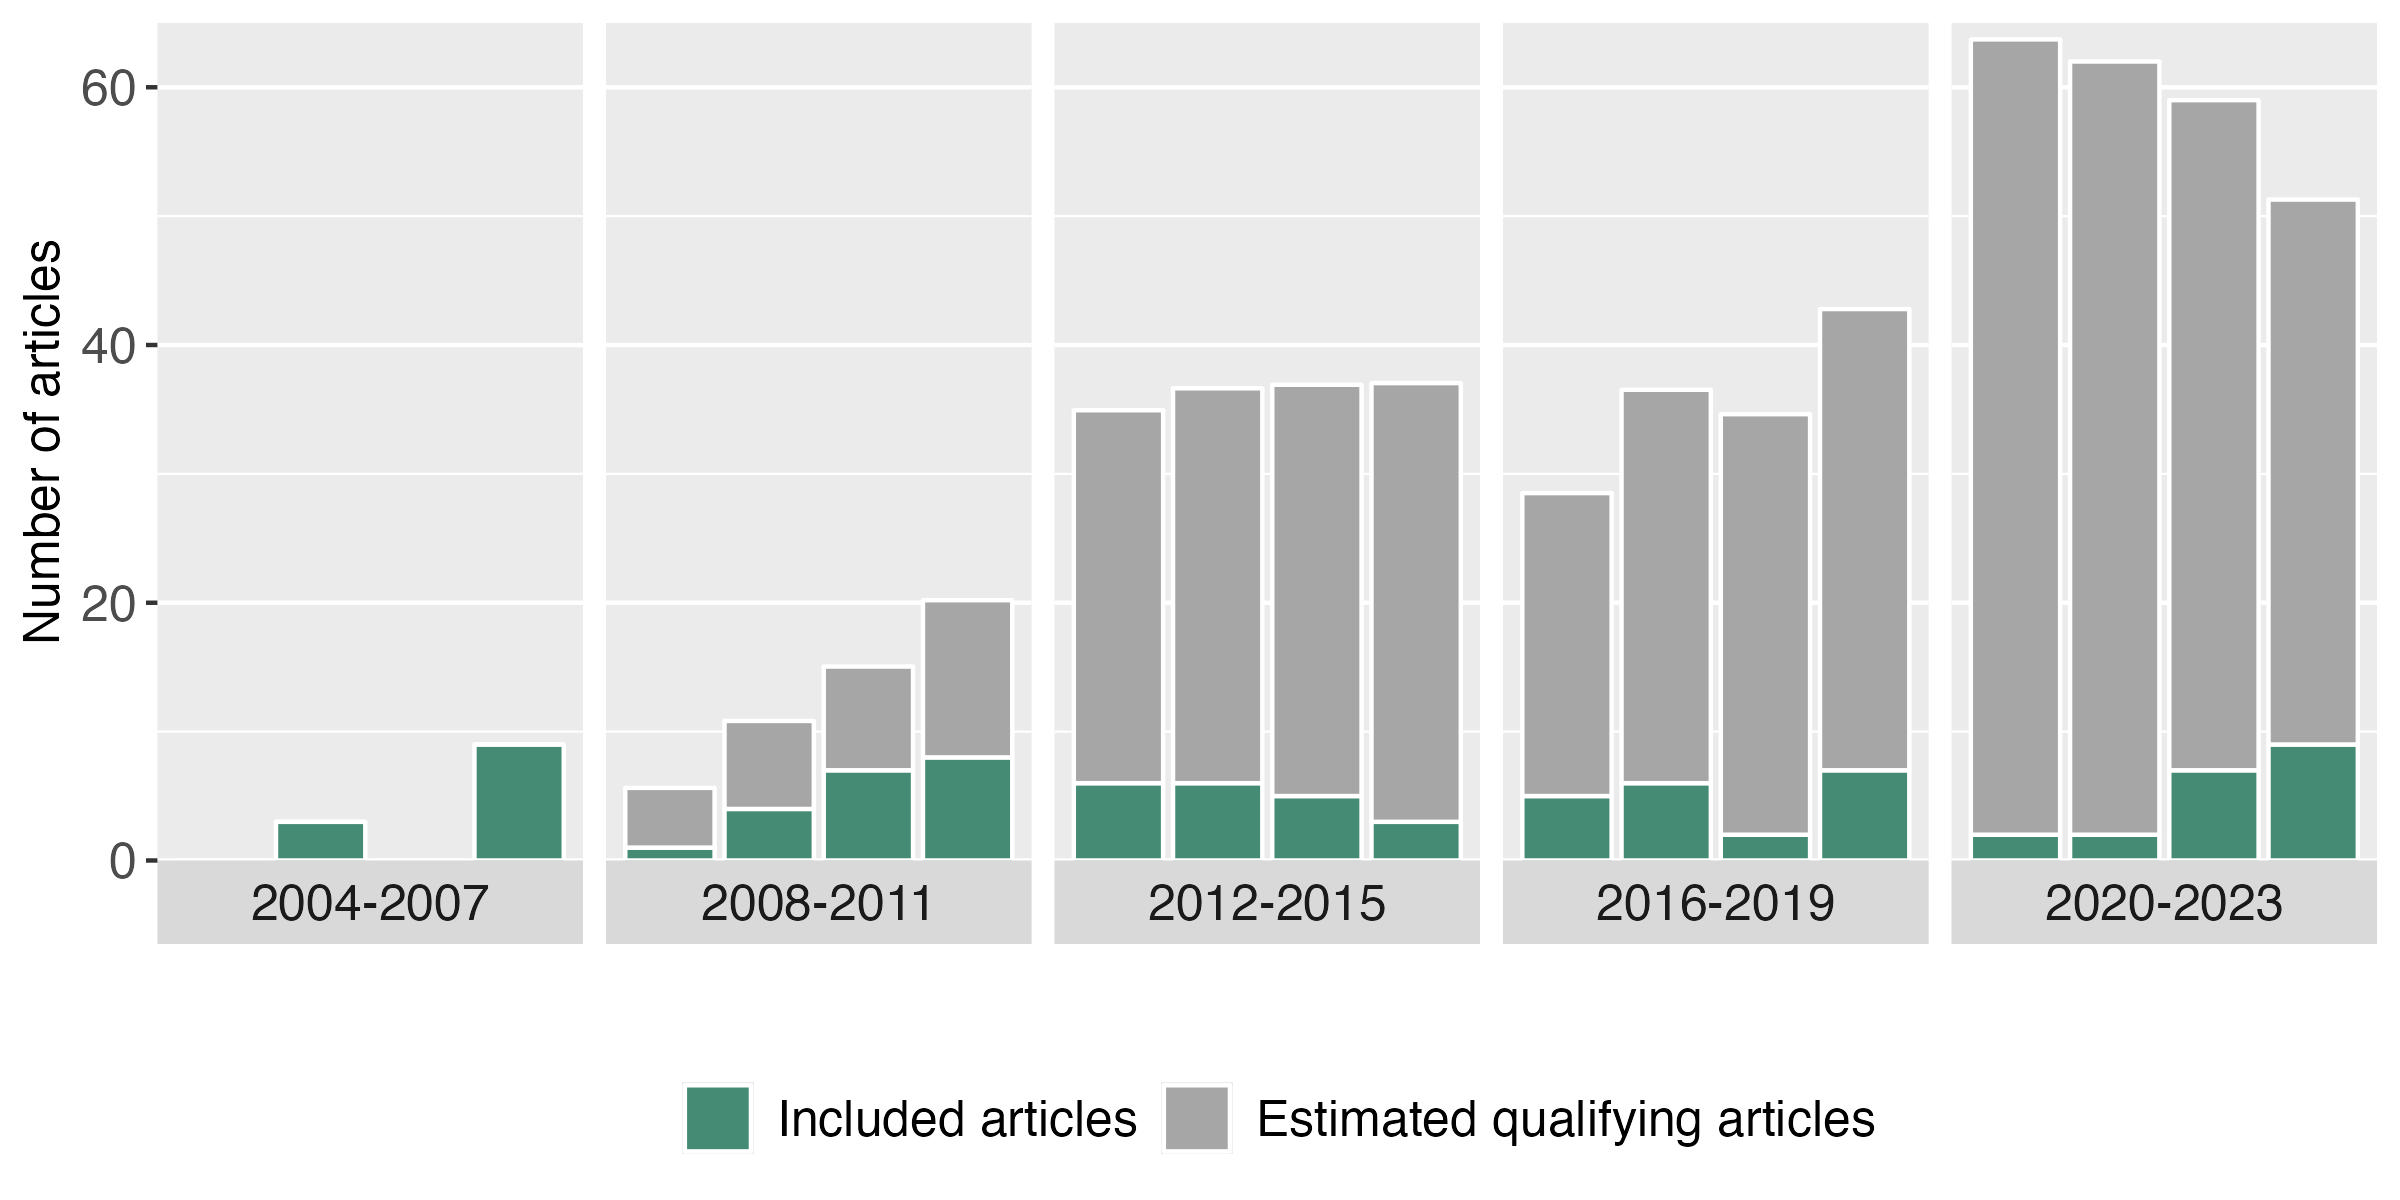
\includegraphics{Figures/CoveragePlot.jpeg}

}

\caption{\label{fig-coverage}Bars indicate the 92 articles included in
our review as a proportion of the estimated number of published articles
fitting DOMs, based on the qualification rate for articles in each
strata. The proportion of articles included from each strata were as
follows: 12.5\% from 2005-2008; 24.4\% from 2008-2011; 42.6\% from
2012-2015; 35.1\% from 2016-2019; and 57.1\% from 2020-2023.}

\end{figure}%

Articles included in our review demonstrate considerable diversity in
scope, scale, and objectives. A selection of key attributes of these
studies is presented in Figure~\ref{fig-StudyDetails}, and we provide
notable examples of DOMs throughout this section to highlight how some
this variation appears in practice. Study systems included in our sample
are globally distributed; while a majority use data collected in the
United States of America, representatives are included from all
geographic realms and an exceptional diversity of ecosystems. A
particularly notable aspect of these study areas is their variation in
size, which ranges from the hyper-local to the continental scale. The
smallest study locality included in our sample studied insect occurrence
in a rainforest plot less than one square kilometre, while the largest
analysis modelled avian range shifts across the entire eastern half of
the United States (Basset et al., 2023; Clement et al., 2019).

The temporal scale of studies shows similar variability. The duration
between first and last survey ranging from under one month to forty
years, with a median of 6 years. More meaningful for model
interpretation, however, is the duration of the primary occasion, as
this is presumed to be the temporal scale at which changes in occupancy
are observed. Most applications describe the primary occasion as a year,
although some studies divide years into multiple primary occasions to
describe seasonal variation in occupancy. In the most extreme cases the
primary occasion may be as brief as a week, capturing much finer scale
changes in occupancy. These shortened-season occupancy models are most
common with camera trapping or acoustic monitoring data, which can be
arbitrarily divided into primary and secondary sampling occasions. This
is seen in Kleiven et al. (2020)'s study of rodent and mustelid
interactions using camera trap data, where the primary occasions are
less than one week in length. On the other end of the spectrum, some
studies modelled primary occasions which were decades apart and
represented generational changes in occupancy. This is illustrated in
Couturier et al. (2023)'s study on long-term otter recovery in France,
which used data from two primary occasions: one in 2003 and one in 2012.

DOMs have been used to study a variety of different species, though the
majority of studies have been conducted on data for vertebrate taxa.
They have been less frequently applied to non-animal organisms, perhaps
due to a reduced emphasis on imperfect detection outside of the wildlife
modelling community. However, there are exceptions --- Belinchón et al.
(2017) fits a DOM to lichen data, and Cook et al. (2022) uses them to
model the spread of chronic wasting disease. The latter's application to
disease dynamics is not unique, and DOMs have been touted as a valuable
tool for modelling disease dynamics. Mores et al. (2020) and
Padilla-Torres et al. (2013) have each used DOMs to model mosquito
dynamics as a human disease vector, and Bailey et al. (2014) discusses
the concept of applying the DOM to the spread of chytrid fungus in
amphibian habitats. The vast majority of applications have been fit for
terrestrial species, though there have been a limited number of studies
on aquatic systems, including Fisher et al. (2014)'s application to
invasive salmon, Falke et al. (2012)'s on Great Plains stream fishes,
and Pendleton et al. (2022)'s on whale occupancy dynamics.

While most articles in our sample fit a model to a single species, 41
fit models to multiple species either as independent models or
explicitly multi-species implementations. The multi-species models use
various extensions of the conventional DOM, including hierarchical
models which fit hundreds of species in a single implementation with
species-level effects(Dorazio et al., 2010; Hendershot et al., 2020), as
well as explicit interaction models which estimate conditional
occupancy, colonisation, extinction, and detection probabilities (Fidino
et al., 2019; Lesmeister et al., 2015). While they did not fit
multi-species models, several other authors fit large numbers of
independent models to different species (Otto \& Roloff, 2012; Peach et
al., 2019). Working with large numbers of taxa does raise additional
challenges, as the level of complexity which can realistically be
considered for each individual taxon is likely to be reduced for the
sake of practicality.

\begin{figure}

\centering{

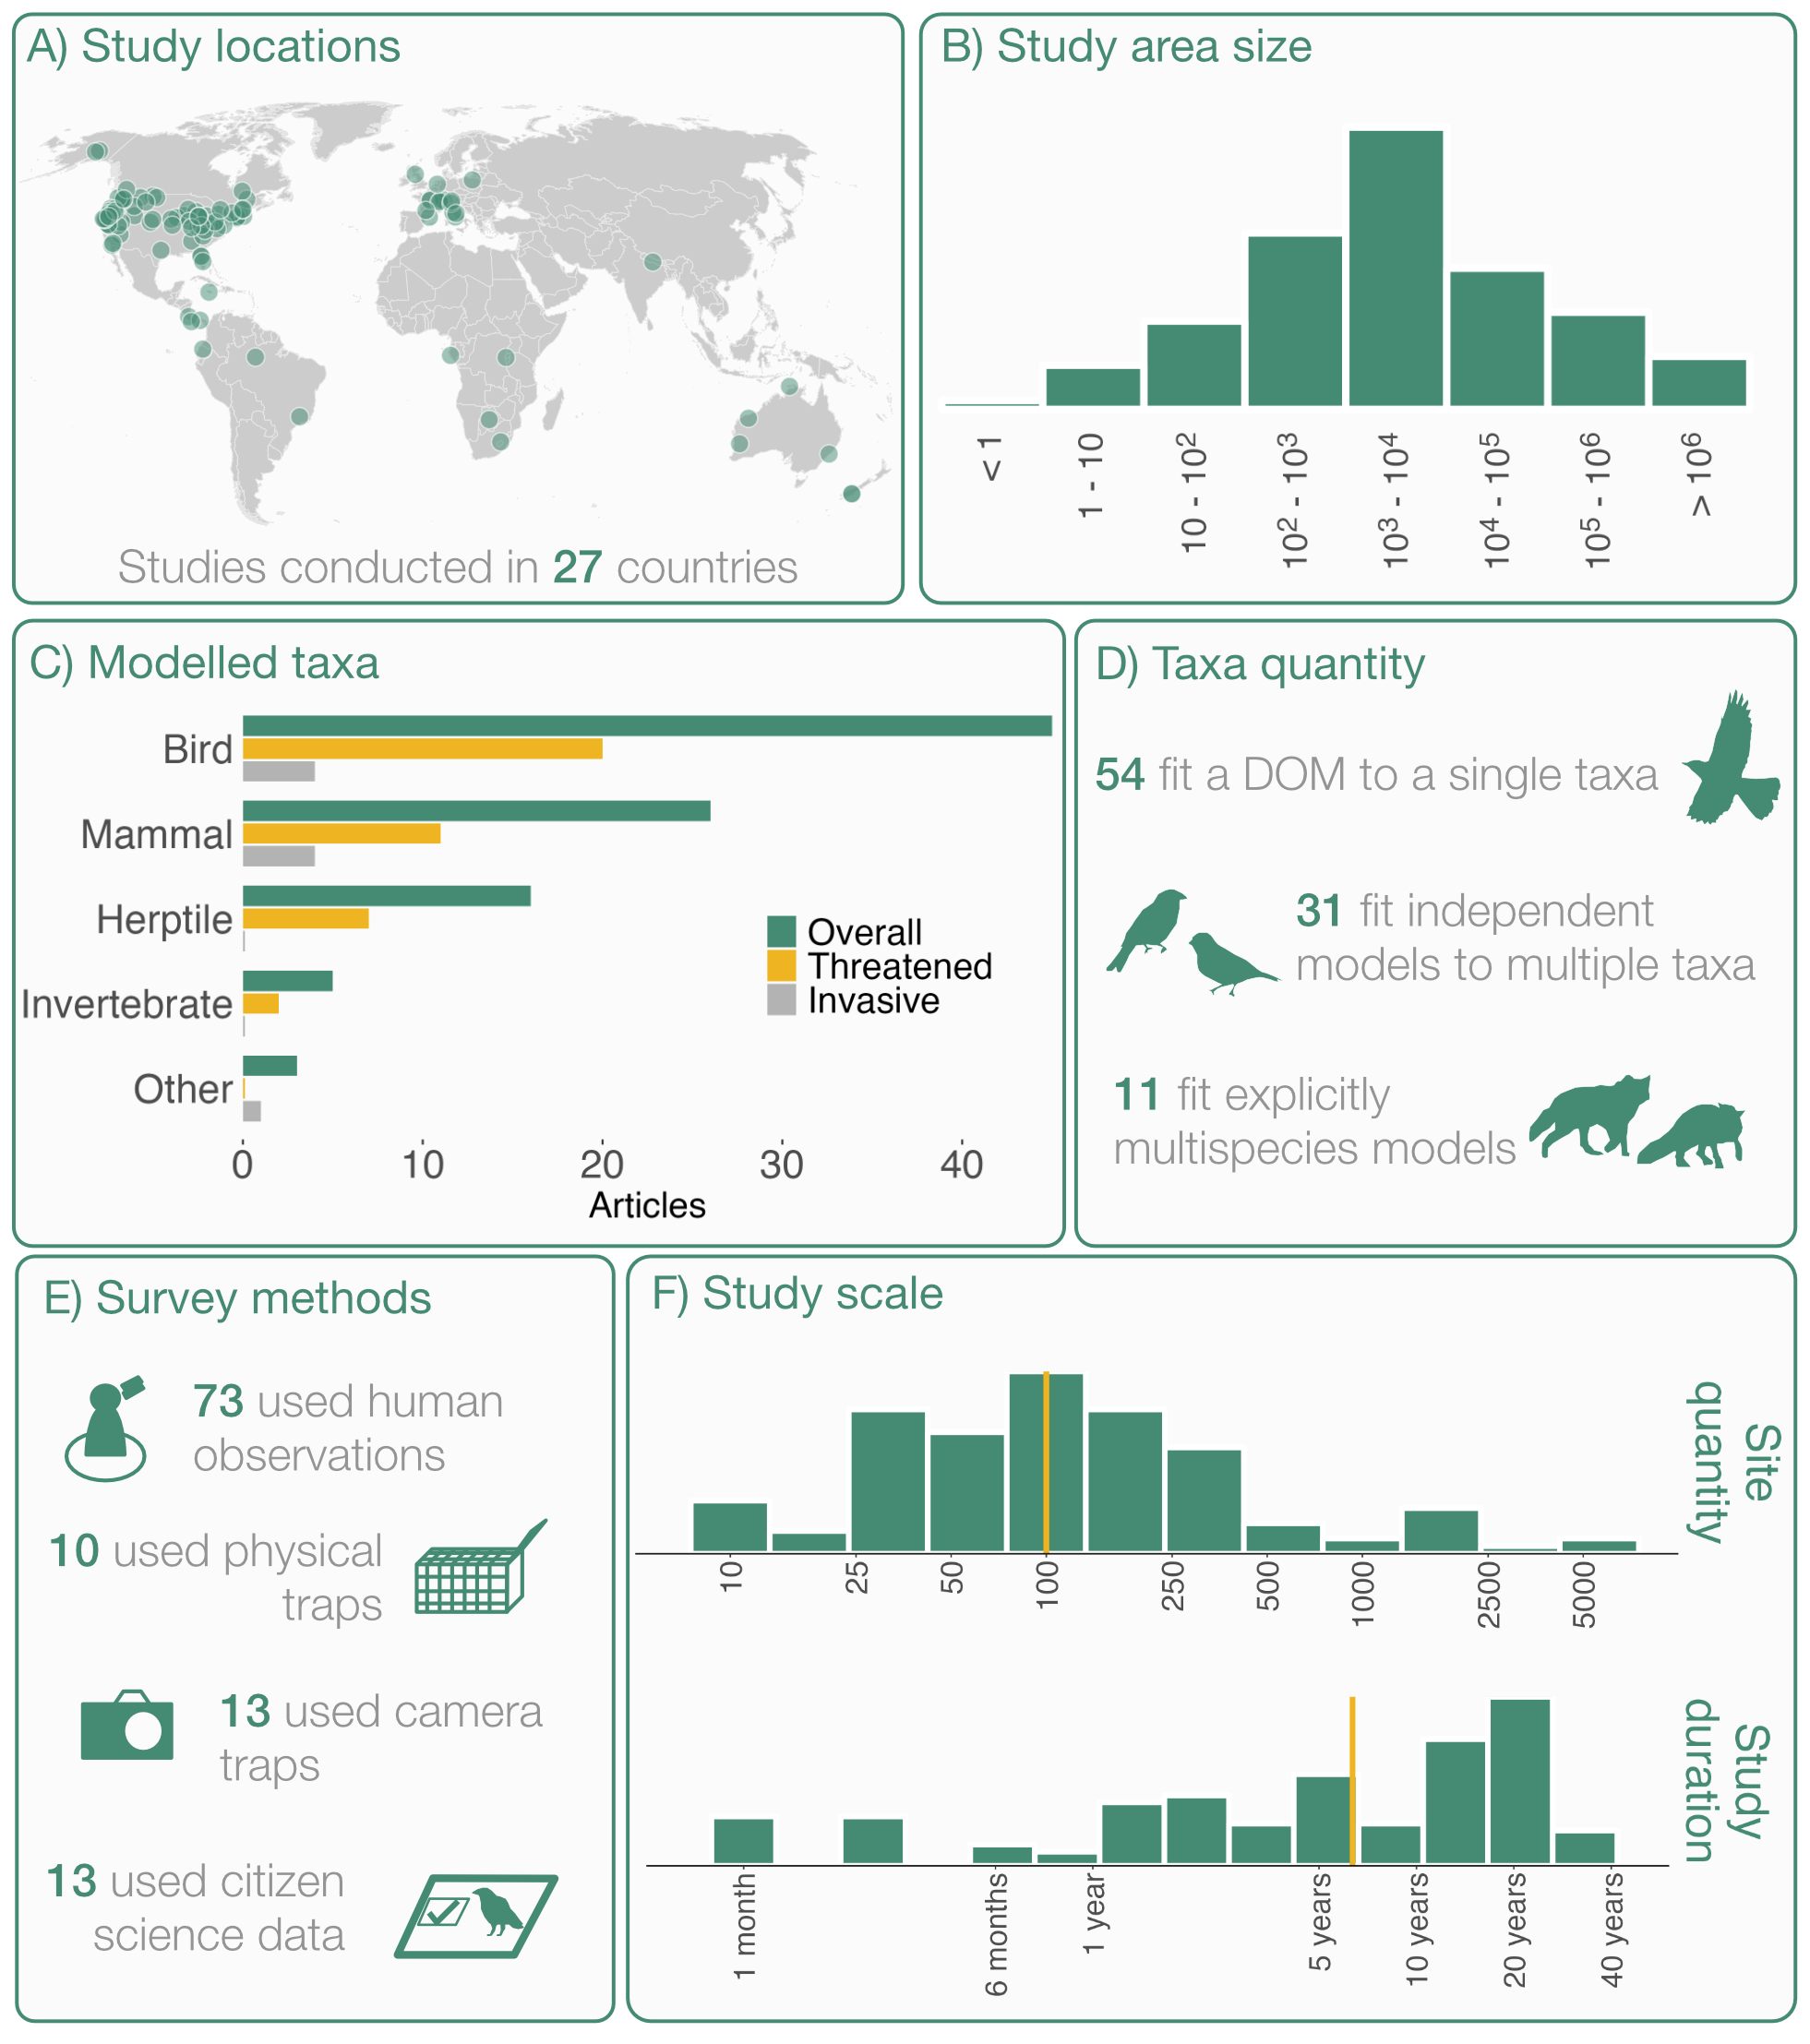
\includegraphics{Figures/ReviewBox.png}

}

\caption{\label{fig-StudyDetails}A) Study areas: Data for a majority of
studies were collected from study locations in the United States. The
size of study areas was log-normally distributed, with the median study
area falling between 1000 and 10000 square kilometres. B) Study taxa:
Most species modelled in our sample were terrestrial vertebrates
including birds, mammals, or herptiles. 55 articles fit models to only a
single taxa, 30 fit independent models to multiple taxa, and 11 fit
multi-species models with explicit interactions between taxa. C) Survey
methods: Approaches to data collected were varied and included
conventional surveys like point counts and transects as well as more
modern methods like camera traps and acoustic monitors. 13 articles
incorporated data from citizen science projects. Project scale was also
variable, with the median study running for 6 years and covering 101
sites.}

\end{figure}%

The presence/absence data required for DOMs has come from a breadth of
different sources and detection methods. In our sample 79\% of articles
used human observational data, 9\% used live-trapping methods, and 14\%
used detections from camera traps. Several articles also use
citizen-science data to build detection histories, including Zuckerberg
et al. (2011)`s model using bird-feeder data and Warrier et al. (2020)'s
using citizen reports of tiger signs. Using citizen-science data may
require additional consideration of assumptions (particularly
false-positives), as discussed in greater detail by Cruickshank et al.
(2019). Within these broad categories of detection method there is
additional diversity, with several studies using unique survey methods
determining the presence of a species at a location. For example, in the
only application of a DOM for a marine species in our sample, Pendleton
et al. (2022) uses aerial transects broken up into grid cells to observe
whale occupancy; and Marescot et al. (2020)'s fits a unique
'multi-species' model treating poachers and using ranger reports to
create detection histories.

Notably, many of these studies use data which were not originally
collected in a robust design framework for occupancy modelling. In these
articles, authors formatted their data into a hierarchical format
post-hoc using a variety of methods. Some defined primary seasons as a
discrete time interval, treating all surveys occurring within the season
as secondary occasions; others defined sites as larger grid cells,
treating any survey falling within the grid as a spatial replicate.
These manipulations permit authors to use data which far predate the
DOM, with one study using surveys conducted by Joseph Grinnell in 1908
to model century-long changes in occupancy (Riddell et al., 2021).

Additionally, not all articles rely on a single source of detection data
- some integrate multiple sources of data to maximise sample size,
combining data from camera traps, sign surveys, and citizen science
reports. These integrated detection method models do require additional
care and consideration; users must ensure that different detection
methods represent comparable spatial and temporal scales, and that any
variation in perceptibility between detection methods is accounted for
(Pitman et al., 2017; Warrier et al., 2020). A special case exists when
different detection methods are used where one has the potential for
false positive detections; e.g., where less-certain citizen science
detections are combined with certain detections from field surveys. In
this context, the certain detections are used to help account for
false-positive detection probability, as in D. Miller et al. (2011)'s
study integrating GPS collars and hunter reports to estimate wolf
occupancy in Montana.

The flexibility in the data used for DOMs, including the model structure
and the scale of observations, is not amenable to a one-size-fits-all
definition of occupancy. Users of DOMs must carefully consider precisely
what they are modelling and address questions on the scale represented
by their model (Chave, 2013). Intepretation and drivers of occupancy may
differ depending on whether a site is represented by a single point on
the landscape or as a grid cell, with the former likely to depend on
more local, small scale factors rather than landscape-level trends
(Stevens \& Conway, 2019). This is also true for the temporal scale of
occupancy: whether a site is occupied within a week or within a year
leads to vastly different conceptions of occupancy. This idea is
particularly relevant in cases where the selection of season length
\emph{is} to some extent arbitrary, as with camera-trap or bioacoustic
data where continuous recordings can be broken down into distinct
`seasons' of any length. DOMs are well suited to these data types
(Balantic \& Donovan, 2019), and the proliferation of autonomous survey
techniques provides novel opportunities for analysis that is simply not
possible with human-collected data. For example, Kleiven et al. (2020)
and Mölle et al. (2022) divide their camera trap records into seasons of
just a few days. While this provides interesting insights of occupancy
at extremely fine temporal scale, further research may be needed on how
to determine appropriate season and survey durations with respect to
research questions and the closure assumption.

\section{Practices in implementation and model
building}\label{practices-in-implementation-and-model-building}

Building dynamic occupancy models can be a challenging process requiring
careful consideration of which environmental factors to incorporate to
adequately represent occupancy and detection in complex natural systems.
In this review, we have recorded all covariates considered for each
model in our sample. These are summarised in a taxonomy presented in
Table~\ref{tbl-covariates}, which states the proportion of articles
considering each type of covariate in their models, the means by which
that covariate data are collected, and how covariates responses are
represented in DOMs. We further categorise these covariates into two
groups: environmental covariates, which represent plausible ecological
correlates of parameters; and structural covariates, representing
aspects of model form and observation functionally distinct from the
environment. Our findings indicate that users of DOMs have incorporated
an exceptionally wide diversity of covariates in their models --- while
the most common varieties of covariates include aspects of habitat and
land cover, a range of other unique factors were considered by authors
in our sample. Many models incorporate covariates representing aspects
of site geometry and connectivity (37\% of articles), adding spatial
components to these DOMs which bear similarities to related stochastic
patch occupancy models. Notable examples of these spatially-explicit
models include Mortelliti \& Boitani (2007)'s model fit to rodent data
in patchy landscapes and Risk et al. (2011)'s hybrid DOM/incidence
function model used to explore meta-population dynamics of rails.
Several studies also include biotic interactions with other species as
covariates, particularly those which describe taxa threatened by
invasive species. Examples include models with barred owl presence as a
covariate on spotted owl occupancy and models with bullfrog covariates
on native amphibian occupancy, each of which effectively incorporate
species interactions without fitting explicitly multi-species models
(Mangan et al., 2019; Rowe et al., 2019).

\begin{figure*}

\begin{longtable}[]{@{}llrrrrrrrrrr@{}}

\caption{\label{tbl-covariates}All covariates considered for inclusion
in a study were classified into mutually exclusive categories. We
calculate the percentage of articles which include at least one
covariate of a given category on any parameter, Initial Occupancy (ψ1),
Occupancy (ψ), Colonisation (γ), Extinction(ε), and Detection (ρ). We
also present the percentage of all implementations of each covariate
category which are dynamic (varying through seasons) and directly
observed, as well as the percentage of articles which model each
category of covariate as a non-linear relationship or as part of an
interaction with another covariate.}

\tabularnewline

\toprule\noalign{}
\multicolumn{2}{@{}l}{%
\multirow{2}{=}{}} & \multicolumn{6}{c}{%
{Percentage of articles with covariate on parameters:}} &
\multicolumn{2}{c}{%
{Percentage which are:}} & \multicolumn{2}{c@{}}{%
{Articles representing this covariate with:}} \\
& & Any & ψ1 & ψ & γ & ε & ρ & Dynamic & Directly observed & Non-linear
relationships & Interactions between covariates \\
\midrule\noalign{}
\endhead
\bottomrule\noalign{}
\endlastfoot
\multirow{9}{=}{Environmental covariates} & \textbf{Habitat}
\emph{Aspects of habitat and land cover} & 56\% & 41\% & 21\% & 43\% &
48\% & 27\% & 21\% & 14\% & 12\% & 26\% \\
& \textbf{Phenology} \emph{Time-varying elements distinct from sampling
occasions} & 38\% & 1\% & 0\% & 6\% & 5\% & 37\% & 100\% & 0\% & 41\% &
12\% \\
& \textbf{Spatial} \emph{Site geometry, connectivity, or other spatial
elements} & 37\% & 22\% & 36\% & 34\% & 30\% & 11\% & 19\% & 25\% & 18\%
& 21\% \\
& \textbf{Climate/Weather} \emph{Climate, weather, and natural
disasters} & 33\% & 13\% & 14\% & 17\% & 18\% & 22\% & 65\% & 15\% &
33\% & 30\% \\
& \textbf{Topography} \emph{Elements of landscape topography, including
hydrology} & 30\% & 24\% & 36\% & 21\% & 19\% & 8\% & 44\% & 16\% & 26\%
& 19\% \\
& \textbf{Anthropogenic} \emph{Relations to human activity} & 26\% &
19\% & 7\% & 23\% & 21\% & 4\% & 55\% & 4\% & 9\% & 26\% \\
& \textbf{Other environmental} \emph{Other environmental covariate not
otherwise listed} & 21\% & 4\% & 21\% & 5\% & 11\% & 12\% & 77\% & 82\%
& 0\% & 0\% \\
& \textbf{Biotic interaction} \emph{Interactions with other (non-plant)
species} & 16\% & 6\% & 0\% & 14\% & 14\% & 6\% & 73\% & 76\% & 7\% &
21\% \\
& \textbf{Any Environmental} & 91\% & 61\% & 93\% & 74\% & 75\% & 72\% &
42\% & 17\% & 34\% & 28\% \\
\multirow{7}{=}{Structural covariates} & \textbf{Primary occasion}
\emph{Effect of the primary occasion} & 66\% & 1\% & 43\% & 38\% & 38\%
& 62\% & 99\% & 0\% & 15\% & 10\% \\
& \textbf{Observation} \emph{Details on the observation process} & 21\%
& 0\% & 0\% & 0\% & 0\% & 21\% & 91\% & 9\% & 5\% & 11\% \\
& \textbf{Secondary occasion} \emph{Effect of the secondary occasion} &
16\% & 0\% & 0\% & 0\% & 0\% & 16\% & 100\% & 15\% & 14\% & 0\% \\
& \textbf{Species effect} \emph{Species-level effects} & 6\% & 5\% & 0\%
& 5\% & 5\% & 4\% & 0\% & 0\% & 0\% & 60\% \\
& \textbf{Site effect} \emph{Site-level effects} & 3\% & 0\% & 0\% & 2\%
& 2\% & 2\% & 0\% & 0\% & 0\% & 0\% \\
& \textbf{Other structural} \emph{Other structural covariate not
otherwise listed} & 3\% & 1\% & 0\% & 0\% & 0\% & 2\% & 60\% & 60\% &
0\% & 33\% \\
& \textbf{Any Structural} & 82\% & 6\% & 43\% & 42\% & 42\% & 81\% &
87\% & 4\% & 15\% & 12\% \\
All covariates & \textbf{All covariates} & 99\% & 63\% & 100\% & 85\% &
86\% & 97\% & 46\% & 16\% & 35\% & 26\% \\

\end{longtable}

\end{figure*}%

Covariate data for studies in our sample was either collected directly
by researchers (17\% of environmental covariate data), or derived from
pre-existing remotely sensed datasets (83\%); this of course varies
depending on the category of covariate. Directly collected data can
generally be expected to represent finer-scale factors like prey species
occurrence or details of habitat structure, which can be difficult to
measure remotely but can often be more proximal drivers of occupancy.
These high quality covariates do come with trade-offs, as they can be
expensive to collect and can often preclude projection to locations
where data are unavailable. For projects interested in making these
projections, remotely-sensed covariates are generally more feasible
despite their generally more distal nature (M. P. Austin, 2002). 42\% of
environmental factors and 87\% of structural factors included in
reviewed articles were dynamic covariates which varied through time ---
this again varied with the category of covariate in question, with terms
relating to climate or weather most frequently dynamic and topographic
covariates universally static.

In the standard DOM, covariates for each parameter are most commonly
incorporated via a logistic regression (i.e., a linear regression
through a logit link function). Statistical relationships between
covariates and model parameters are represented as linear terms unless
otherwise specified. Of course, many ecological relationships are
non-linear and require more complex forms to be realistically
represented in a model. M. Austin (2007) discussed the importance of
modelling ecologically-realistic responses to covariates, advocating for
careful consideration of the most appropriate statistical form for
hypothesised relationships. However, linear models are quite flexible,
and non-linear responses can be easily accommodated using polynomial
terms and interactions between covariates. Despite this, in our sample
just 35\% of articles considered using at least one non-linear responses
to an environmental covariate, with the majority of studies representing
all covariates as simple linear relationships. Interactions between
covariates were similarly rare, with only 26\% of studies considering at
least one relationship between terms. The relatively low emphasis on
more complex non-linear responses contrasts with other popular methods
for modelling species occupancy. Many common approaches for SDMs, which
include MAXENT and Boosted Regression Trees, permit considerable
flexibility in the shape of their covariate response curves where
supported by the data (Elith et al., 2008; Merow et al., 2013). This
emphasis on more complex responses in SDMs may be due to their typically
larger range-wide scale which encompasses the full species niche, where
environmental relations may be expected to be non-linear. However, as
previously indicated DOMs have been frequently implemented at similarly
large spatial scales where the same assumptions should exist and similar
responses might be expected. Similar concerns exist for the relatively
low level of interactions between covariates: while they should not
necessarily be used liberally, where these exist their exclusion can
influence model performance (Guisan et al., 2006).

In addition to the types of covariates considered for modelling we also
measured the size of the candidate covariate pool in each reviewed
study, tallying the number of environmental and structure covariates
which were available for use on each parameter (
Figure~\ref{fig-covariates}). This is an area of considerable variation
in modelling practices --- the number of covariates considered for each
parameter ranges from 0 (effectively modelling the parameter as a
constant) to over 40 possible factors.

\begin{figure}

\centering{

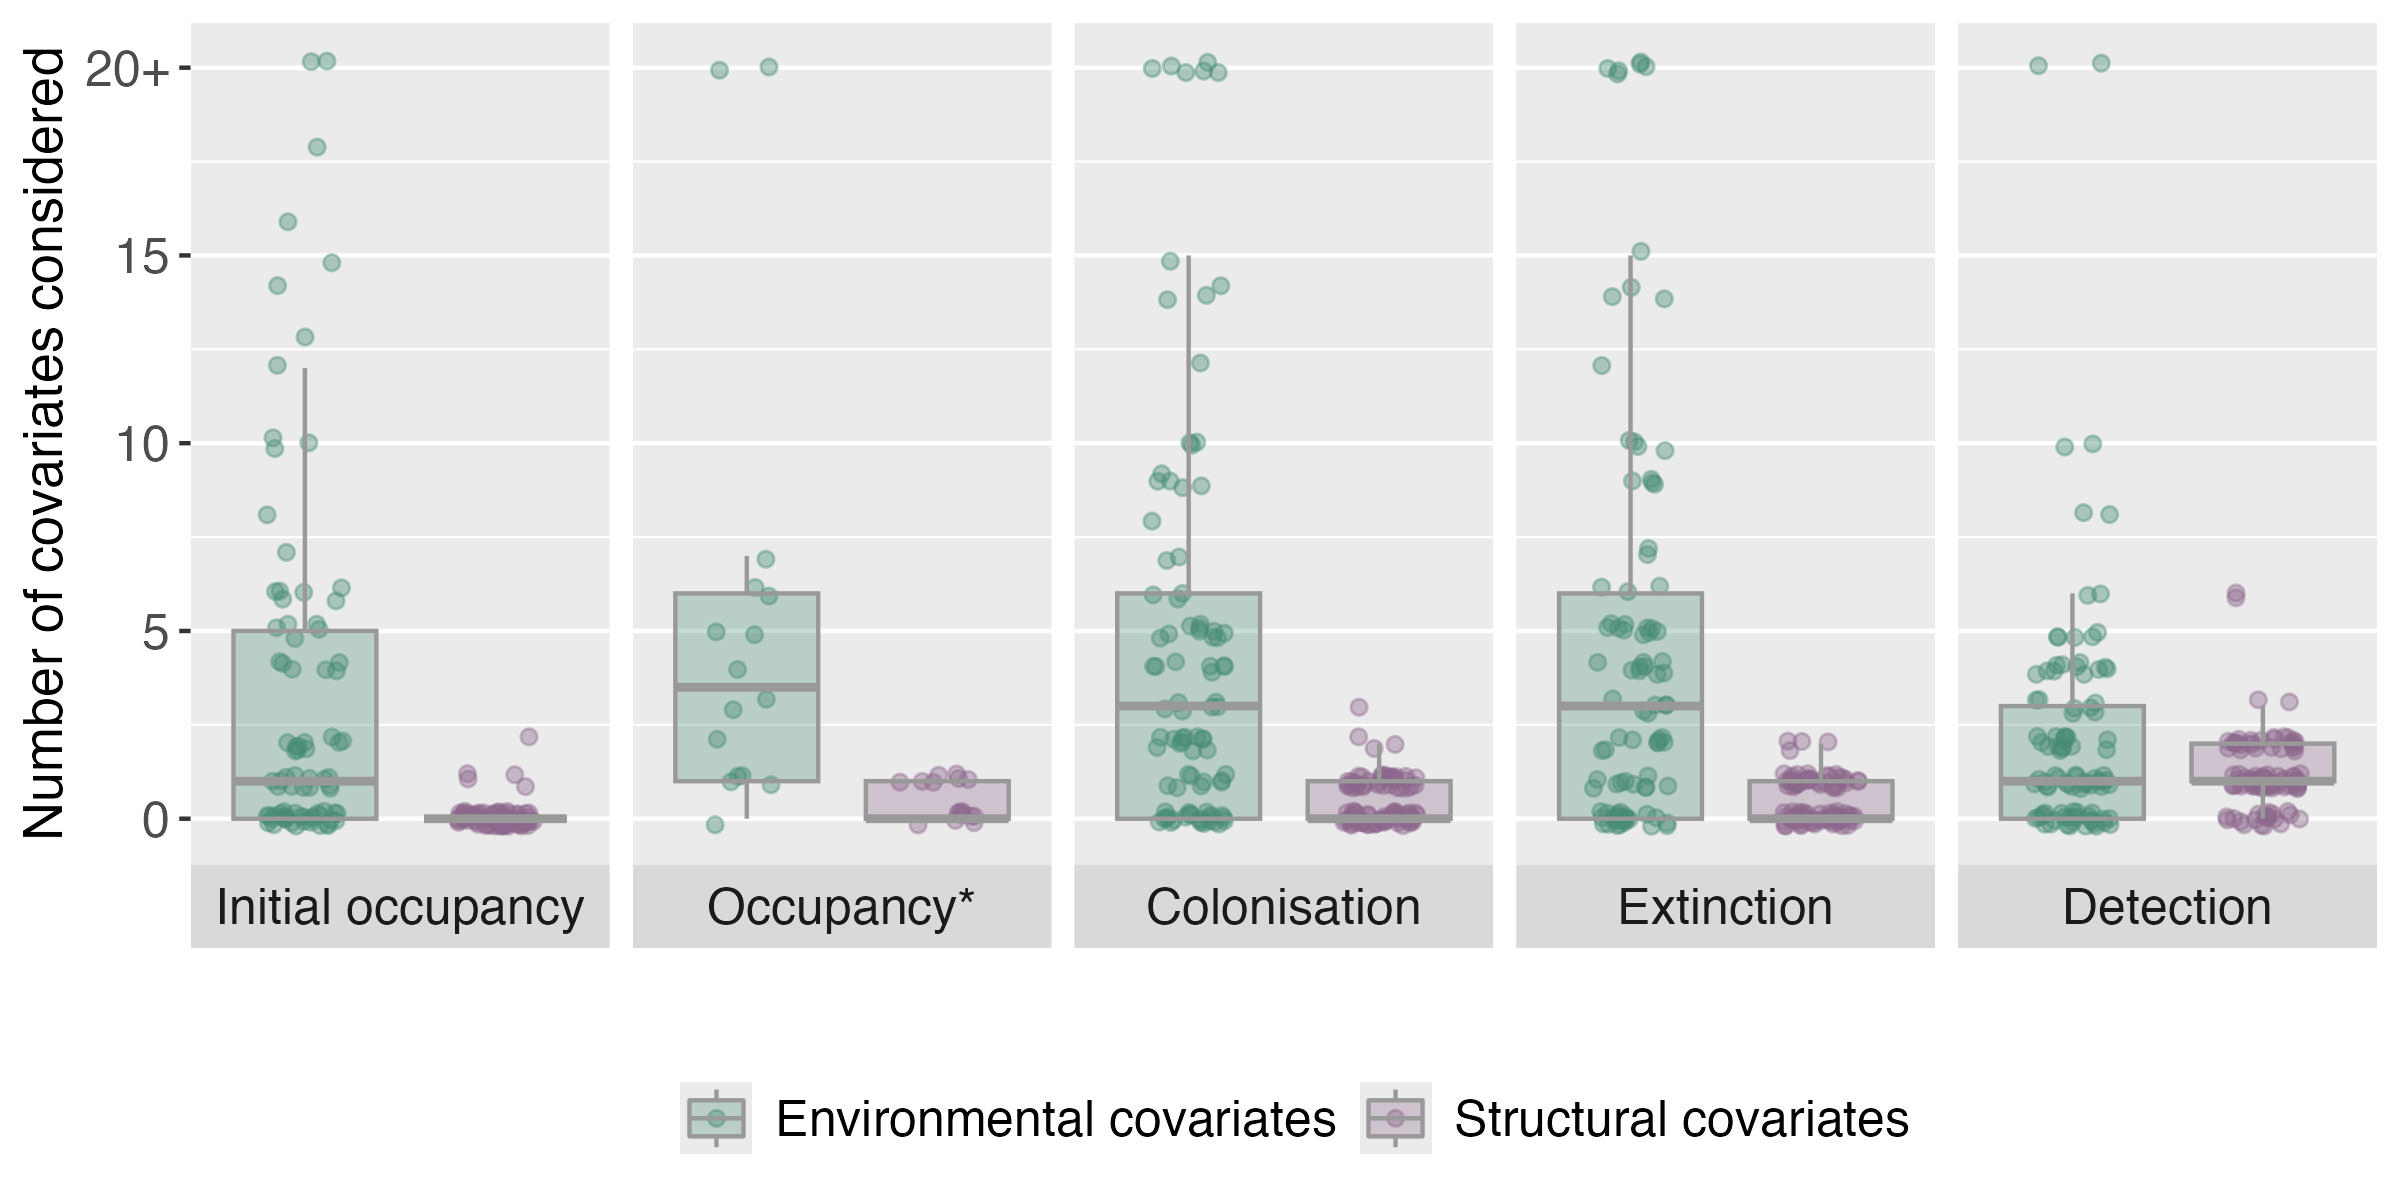
\includegraphics{Figures/CovParamPlot.jpeg}

}

\caption{\label{fig-covariates}The number of covariates considered for
each parameter across all studies in our sample. `Occupancy' given here
represents an alternative parameterisation of the DOM which jointly
estimates Occupancy for every season, Colonisation, and Detection, where
Extinction is a derived parameter; this differs from the more popular
Initial occupancy/Colonisation/Extinction/Detection parameterisation.
Here, a `covariate' is defined as each distinct covariate considered for
inclusion. Linear and quadratic representations of the same covariate
are counted as 1 covariate.}

\end{figure}%

The median number of covariates varies strongly by parameter, with
transition probabilities (colonisation and extinction) more likely to
consider a broader range of environmental covariates relative to initial
occupancy and detection. The lack of any covariates considered for
initial occupancy in many studies (37\% of articles) is particularly
notable --- unless a study is conducted at very small extents or study
sites are truly uniform in their suitability, one would expect some
amount of non-random variation in occupancy probability across any study
system that will not be captured when representing initial occupancy as
a constant. Omission of the factors which drive occupancy is a known
source of bias in static SDMs (Barry \& Elith, 2006), which the initial
occupancy component of the DOM conceptually resembles. Furthermore, any
bias in occupancy estimation in the first time-step will perpetuate into
future seasons due to the DOM's Markovian nature with implications for
the reliability of model outputs. Detection probability is also
typically represented with low quantities of environmental covariates.
Recall that detectability is dependent on not only observation factors,
but also by drivers of abundance and species use; the low number of
candidate covariates here relative to colonisation and extinction raises
additional questions on whether this variation is always appropriately
captured in models.

To this point in our review, we have discussed only the covariates which
were \emph{considered} for inclusion in DOMs without regard for which
terms were actually \emph{included} in the final models used by authors
to make their inference. Identifying the `best' model from a range of
possible candidates can be a challenging process, especially for
hierarchical models like DOMs (Doherty et al., 2012). Consider that the
quantity of candidate models involving up to \emph{n} covariates on
\emph{p} parameters can be given by \((2^n)^p\); where a simple
single-parameter may have up to 64 possible combinations of 6
covariates, a 4-parameter dynamic occupancy model would have 16 million
combinations. This explosion of candidate models generally precludes
exhaustive comparisons of possible models and requires a reduction of
the models tested. Models in our sample include both Frequentist (n =
70) and Bayesian (n = 22), which differ considerably in their manner of
implementation. A summary of modelling practices in DOMs is given in
Table~\ref{tbl-modelling} below.

\begin{longtable}{l|rrr}

\caption{\label{tbl-modelling}Modelling practices in dynamic occupancy
models, subset by frequentist or bayesian implementations. The median
covariate count presented here represents the median quantity of
covariates considered for each model parameter across the studies in our
review. The model selection methods represented in this table are
non-exclusive and some articles employ multiple approaches.}

\tabularnewline

\toprule
\multicolumn{1}{l}{} & Frequentist & Bayesian & All models \\ 
\midrule\addlinespace[2.5pt]
\multicolumn{4}{l}{\vspace*{-5mm}} \\ 
\midrule\addlinespace[2.5pt]
Number of studies & $70$ & $22$ & $91$ \\ 
Median covariates considered per parameter & 3.12 & 2.5 & 2.75 \\ 
\midrule\addlinespace[2.5pt]
\multicolumn{4}{l}{Covariate selection methods} \\ 
\midrule\addlinespace[2.5pt]
\hspace*{11.25px} Prop\_AnySelect & $94\%$ & $36\%$ & $80\%$ \\ 
\hspace*{11.25px} Prop\_Candidate & $43\%$ & $14\%$ & $36\%$ \\ 
\hspace*{11.25px} Prop\_Sequential & $39\%$ & $0\%$ & $30\%$ \\ 
\hspace*{11.25px} Prop\_Simple & $9\%$ & $5\%$ & $8\%$ \\ 
\hspace*{11.25px} Prop\_ModAvg & $71\%$ & $5\%$ & $56\%$ \\ 
\midrule\addlinespace[2.5pt]
\multicolumn{4}{l}{Model evaluation conducted} \\ 
\midrule\addlinespace[2.5pt]
\hspace*{11.25px} Prop\_GOF & $20\%$ & $14\%$ & $19\%$ \\ 
\hspace*{11.25px} Prop\_Eval & $4\%$ & $18\%$ & $8\%$ \\ 
\bottomrule

\end{longtable}

The largest differences between the frequentist and Bayesian models in
our sample lie in their approaches to model selection. Where 94\% of
frequentist models perform some manner of model selection to determine
covariate inclusions for their models, only 36\% of Bayesian models do
so, with the majority instead fitting a single model defined \emph{a
priori}. Methods used for model selection vary considerably both within
and between modelling frameworks. For frequentist models, the most
popular and conventional approach to model selection as used in 43\% of
articles involves the creation of a fully pre-defined model set
containing some number of hypothesis candidate models, where the best
model is selected according to the lowest AIC score. Most frequentist
studies which do not follow this protocol instead use procedural model
selection methods (39\% of articles), where the structure for each model
parameter is fit one-by-one. For example, this protocol might first
identify the best structure for detection probability before moving on
to initial occupancy and so on. A smaller portion of frequentist studies
(9\%) use more unique approaches, fitting simpler models such as single
season occupancy models for candidate covariates to identify the most
informative terms to use in a DOM. Across all frequentist
implementations, 71\% of articles conduct multi-model inference and
model-averaging using AIC weights (Burnham \& Anderson, 2004).

Those Bayesian models which \emph{do} perform model selection tend to
take distinctly different approaches, with largely idiosyncratic methods
across these studies. While direct comparison of model fit is rare, it
is feasible --- Urban et al. (2023) identifies the best model from a
Bayesian candidate set using the predictive performance on both in and
out-of-sample validation data. Another approach used by Cook et al.
(2022) fit a global model including all covariates before removing each
covariate where the 95\% credible interval of the posterior distribution
overlapped zero and refitting the model. Ahumada et al. (2013) takes a
hybrid approach, in which model selection is conducted by a procedural
method in the frequentist framework before refitting the best structure
in a Bayesian model.

Limited research has been conducted on advantages of different methods
for covariate selection in DOMs, and there is surely no one-size-fit all
approach which will be appropriate for all possible use-cases. However,
it is important to consider the implications of the different model
selection approaches in common usage, and research from the SDM
literature highlights how covariate selection can influence our
interpretation of model outputs (Brodie et al., 2020). Within the
occupancy modelling literature, Stewart et al. (2023)'s article on
covariate selection in single-season occupancy model discusses important
attributes of the information-criteria approaches widely used in
frequentist models in our review, noting that these approaches can lead
to inaccurate estimates and influence model inference. Morin et al.
(2020)'s work raises different concerns on procedural model selection
methods, demonstrating how the fine details of modelling protocols can
determine whether the best-fitting possible model is identified and
which covariates appear in final models. The literature on performance
of Bayesian model selection methods is more sparse, although Hooten \&
Hobbs (2015)'s guide to Bayesian model selection in ecology is a
valuable resource for possible methods of fitting those models.

With few exceptions, most of the model selection methods identified in
our review are designed only to identify the best model of those
considered, and do not necessarily guarantee that selected models are
well-fit to the data. Assessment of the performance of DOMs generally
requires additional steps, and the best ways to achieve this are not
necessarily clear. There is no broadly-accepted goodness-of-fit test for
dynamic occupancy models, although MacKenzie \& Bailey (2004) describes
an approach for single-season occupancy models using a parametric
bootstrap which can been extended to DOMs; this test is implemented in
the \emph{AICcModAvg} and \emph{unmarked} R packages. Kéry \& Royle
(2021) describe the test and present an alternative based on separately
assessing fit to static and dynamic components of the model. In Bayesian
implementations, posterior predictive checks offer means to assess model
fit (Gelman, 2014). Broms et al. (2016) discusses possibilities for
model evaluation in the Bayesian context focusing on single-season
multi-species occupancy models but extensions of their approach may also
be applicable to the DOM. As in other hierarchical models, model
evaluation for DOMs can in general can be difficult and somewhat
uncertain compared to other model types, as the primary response
variable of interest (species occupancy) is a latent variable where the
true state is generally not known. Predictive performance evaluation is
thus typically based on \emph{observed} occupancy data, where a DOM is
used to simulate detection histories to be compared with field survey
results.

Perhaps as a result of this uncertainty, assessment of model fit and
model performance was rare amongst the articles in our sample. Only 19\%
of studies tested for goodness-of-fit, and just 10\% calculated
predictive performance. These rates are considerably lower than for
models like SDMs; for which M. B. Araújo et al. (2019)'s review of
applications found closer to 50\% articles testing both fit and
performance.

\section{Modelling objectives}\label{modelling-objectives}

Studies in our sample were classified according to their objectives as
stated by authors to explore the use-cases which DOMs have been applied
for. These objective categories were non-exclusive, and many studies
fell into multiple categories; the frequency at which studies pursued
each of these objectives is shown in Figure~\ref{fig-objectives} A.
Across our study period DOMs have been frequently employed to observe
trends in species occupancy, to explore relationships between
environmental factors and occupancy, and, increasingly often, to make
predictions of occupancy spatially to unsurveyed locations or temporally
to hypothetical future conditions. Within each of these broad categories
lies even more variation in objectives, emphasising the DOM's
flexibility as a tool for making ecological inference in diverse
contexts.

Many articles in our sample used the DOM seeking to monitor trends in
occupancy state through time. These studies include Ahumada et al.
(2013)`s paper assessing populations trends of 13 forest mammals and
Scott \& Rissler (2015)'s assessment of the conservation status of the
endangered flattened musk turtle. These studies offer valuable insights
on the state of species across landscapes and through time,
demonstrating DOMs' suitability for many monitoring oriented projects
--- including those where many species need to be assessed at once.
Other articles were more focused on examining the factors which
influence species occupancy, either testing a pre-specified hypothetical
relationships or taking a broader tack to identify drivers of occupancy
without preconception. The distinction between the two is important, as
it guides which covariates may be considered and how model selection may
be used to fit models. Many of these studies target core conservation
priorities for their focal species, like Olson et al. (2005)'s early DOM
assessing the influence of barred owls on threatened spotted owl.
Explorations of these pivotal relationships are important for guiding
management action, and may also be used to test the effectiveness of
these actions as in K. E. Miller \& Brown (2023)'s study on American
Kestrel nest boxes. In scenarios where less is known about species
habitat preference, DOMs may be used to examine the influence of a wider
variety of factors as illustrated in Huber et al. (2017)'s study testing
the relative influence of dozens of habitat covariates on Wood warbler
occupancy. In recent years, increasing numbers of articles have used to
DOM to generate predictions of species occupancy. As examples, McGowan
et al. (2020) provides projections for the threatened Black rail under
multiple management scenarios, and Pollentier et al. (2021) generates
maps of distributions resembling those made with SDMs, outputs which can
immediately be used by managers to inform action.

\begin{figure}

\centering{

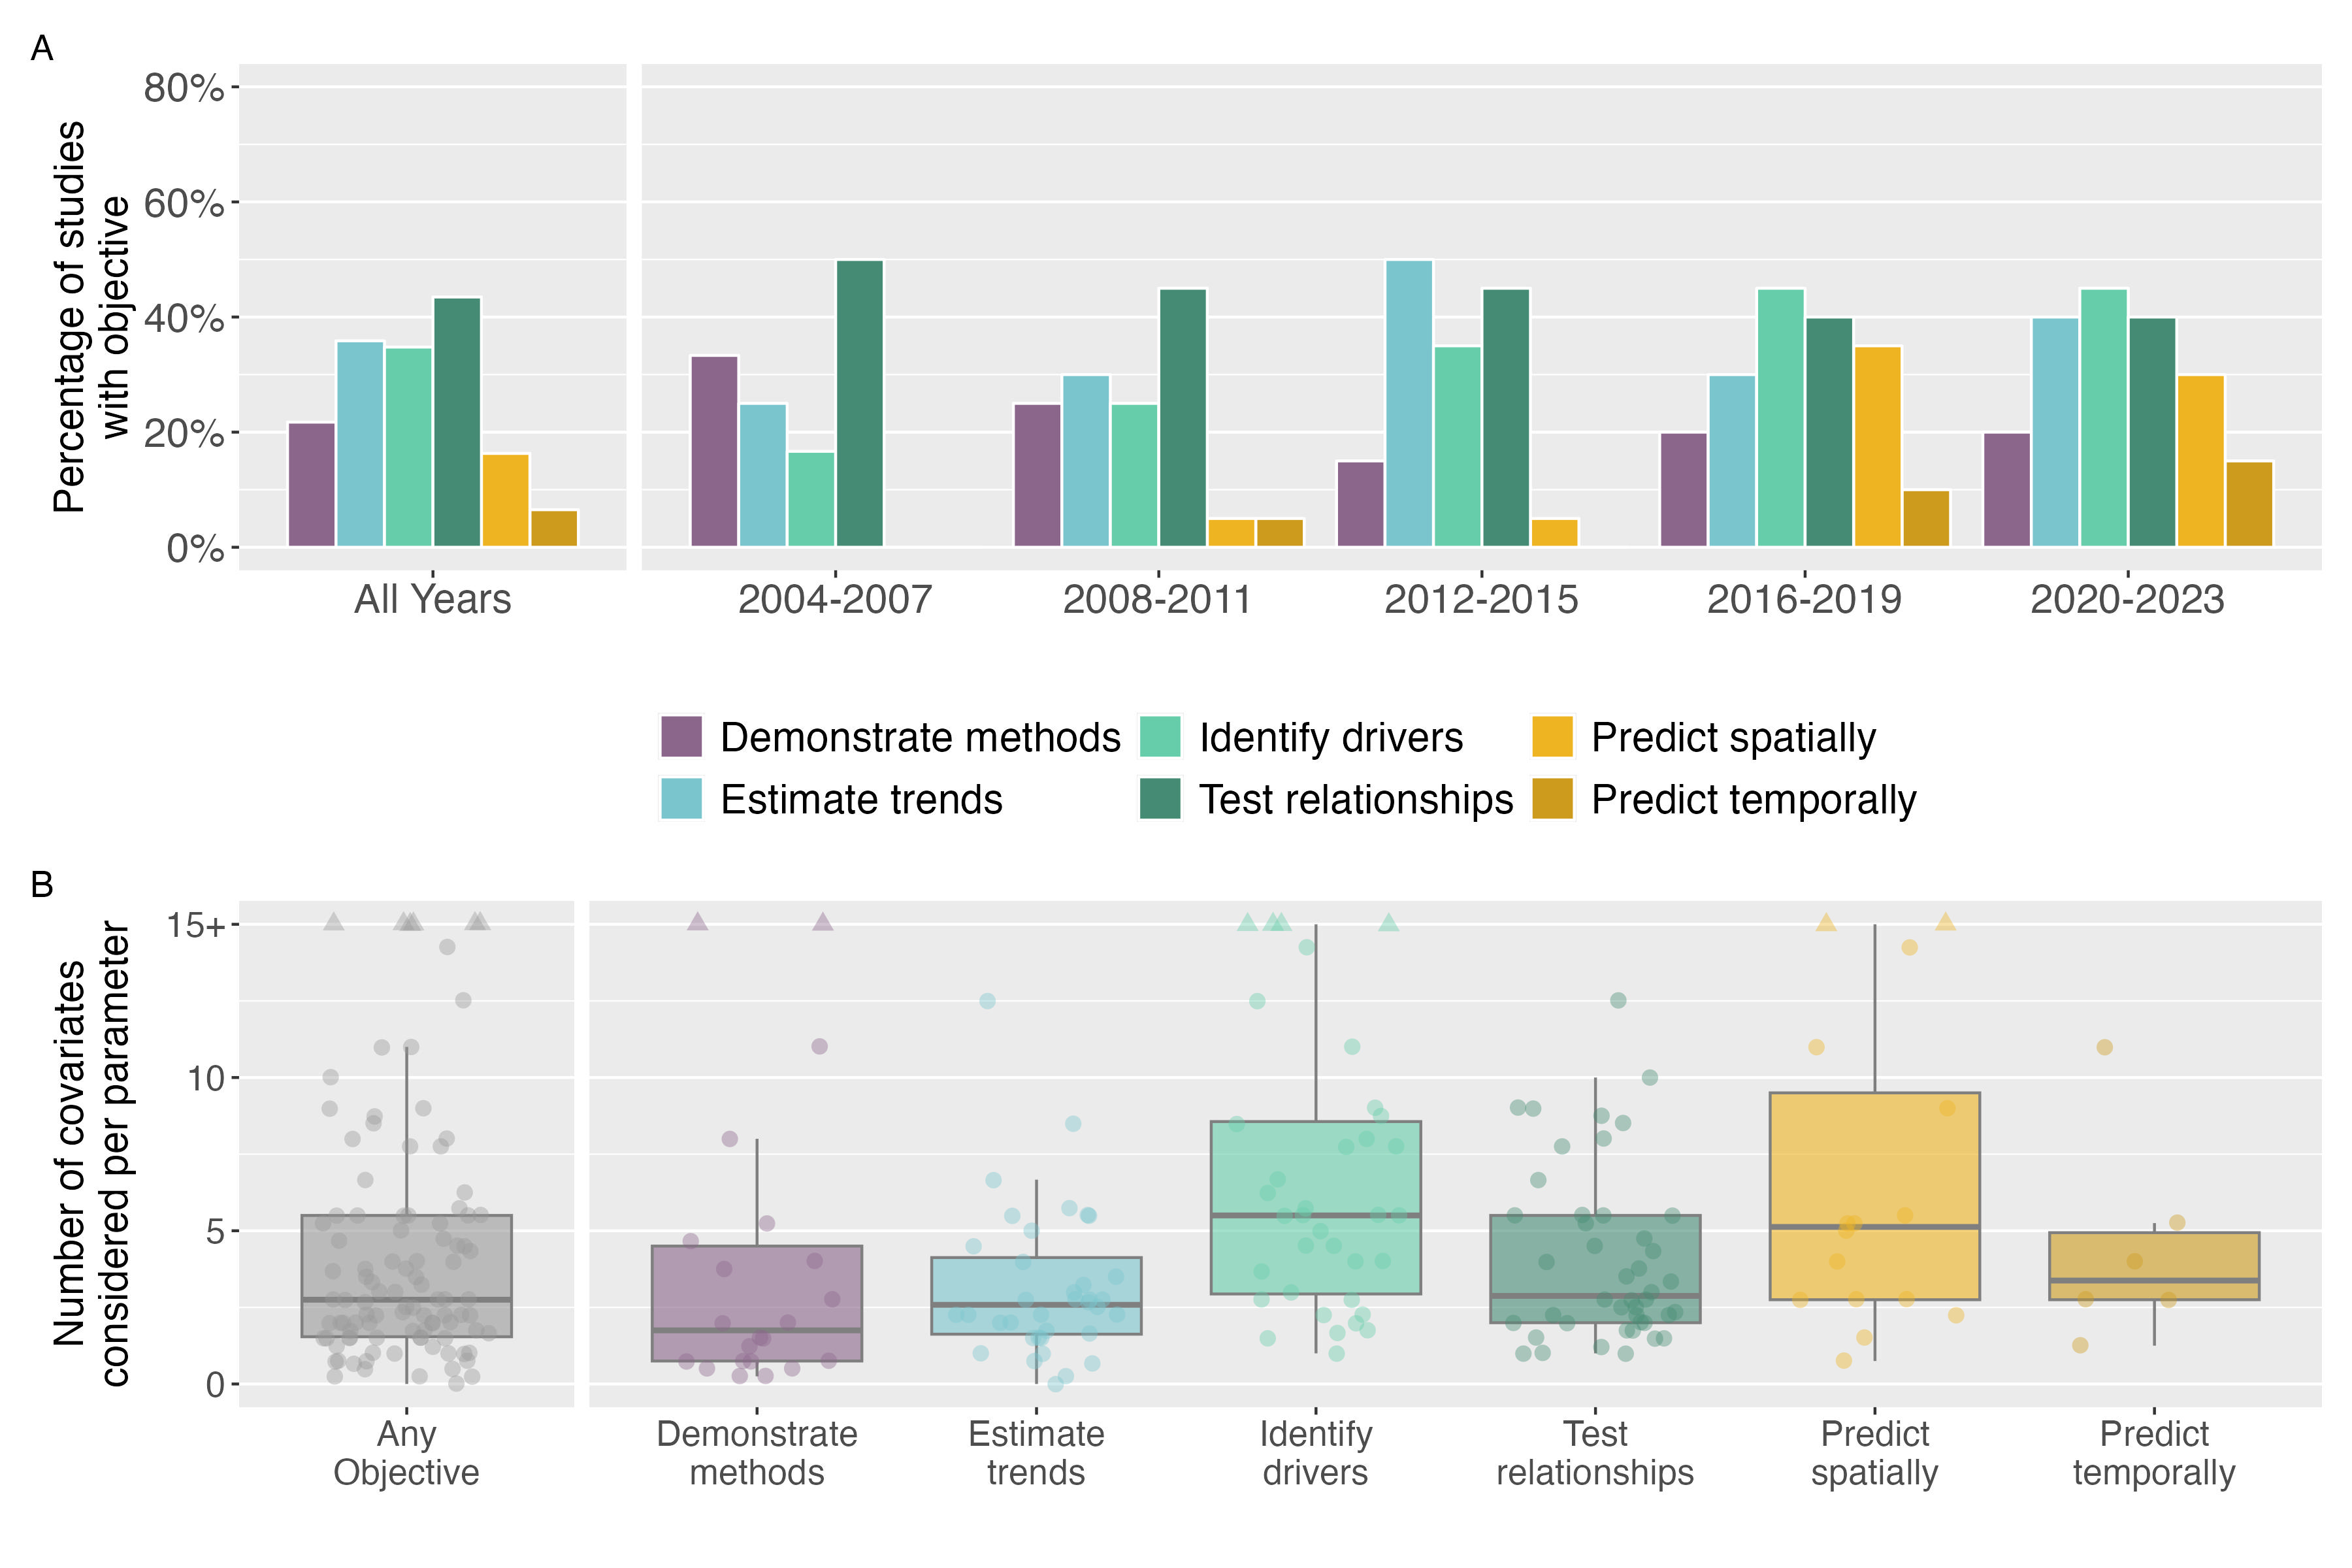
\includegraphics{Figures/ObjectiveFigure.jpeg}

}

\caption{\label{fig-objectives}A) Shows the proportion of articles in
each year-strata and across all years which match each of six
non-exclusive objective categories. B) Shows the quantity of covariates
considered per parameter for models which pursued each objectives.
Studies focused on methods development typically considered the fewest
covariates, where those attempting to identify the drivers of occupancy
considered the most.}

\end{figure}%

The objectives of studies fitting DOMs strongly inform approaches to the
model building process, particularly with respect to covariate
selection. Figure~\ref{fig-objectives} B shows the quantity of
covariates considered for models applied to each of our objective
categories, and the differences between objectives are apparent. Not
unexpectedly, articles which focused on describing new methods for DOMs
had fewer covariates than those studies focused on more applied
objectives. However, differences persist between those articles
observing trends, identifying trends in occupancy, testing
relationships, and making predictions.

\section{Synthesis and key
priorities}\label{synthesis-and-key-priorities}

Approaches to building any type of model will necessarily depend on the
possibilities of the data at hand and on the priorities of the
model-builder. This precludes any prescription of the `best' way to
build a model, however, there are still important discussions to be had
on decisions made in the modelling process. One aspect of fitting DOMs
meriting broader discussion revolves around `model complexity,' and how
much must be incorporated into models to reliable model species
occupancy under different contexts and use cases. Complexity is a broad
term which encompasses many aspects of a model (Merow et al., 2014), and
opinions on simplicity versus complexity in ecological models can be
divisive. Where some advocate for the simplest possible models, arguing
that they are most generaliseable; others insist that overly-simple
models cannot adequately represent the most important drivers in a
system (Evans et al., 2013; Lonergan, 2014). By their nature DOMs are
somewhat more complex than simpler models for studying occupancy thanks
to their hierarchical structure, attributes which are necessary to
control for detectability and to capture occupancy dynamics. Within this
structure, however, further complexity is to some degree up to the
modeller: one can choose how many covariates to consider for inclusion
on the various parameters, and how to represent the nature of the
relationship between those covariates and parameters. Research from SDMs
indicates that allowing for more complex relationships can improve model
performance in predicting occupancy (Valavi et al., 2023), an
increasingly popular use-case for DOMs. Within the DOM framework, there
are exciting developments on that front --- Joseph (2020) presents a
novel neural-network occupancy model which allows for exponentially
higher levels of complexity and may offer improved performance for
prediction-oriented studies.

Generally speaking, covariate selection seems to be a particularly
important area for further investigations into building DOMs. In our
review, we see little consensus around which approaches are most
applicable for any given use case, and existing work on covariate
selection in DOMs raises concerns on whether common methods always
produce the most suitable models. This is true for both frequentist and
Bayesian implementations, and comparative research on covariate
selection under both frameworks may help to inform model users on which
method may be most appropriate for their use-cases. In a similar vein,
the low number of articles in our review which conducted model
evaluation or assessed model fit raises different questions. While the
appropriate method of model evaluation may depend on data availability
and research objectives, assessing models by some method is generally
important to understand how reliable model outputs may be (M. Araújo et
al., 2005; Guisan \& Thuiller, 2005). Existing uncertainties around
whether current methods are suitable for the task surely discourage
users from calculating these metrics, and further research is needed to
establish trusted practices for assessing the quality of DOMs.

These priorities are particularly important given the frequent applied
objectives of DOM users, tackling challenges which include assessing
critically endangered species (Carvalho et al., 2023), guiding public
health management of disease vectors (Moreira et al., 2016), and
tracking rapidly developing biological invasions (Wood et al., 2020).
DOMs are well suited to these situations, and it is to be expected that
as these types of applications are more commonly attempted understanding
the sensitivity of model outputs to decisions made in the model fitting
process becomes increasingly important. In the two decades since the
publication of MacKenzie et al. (2003) the dynamic occupancy model has
become a widely used tool for ecological inference, with numerous
extensions to the modelling framework further broadening the scope of
questions and use-cases for which it may be applied. Given their
increasing popularity, further research and guidelines around issues of
model building may help to make the DOM format more accessible to
newcomers and support confidence in interpretation of models. Parallels
to existing work in the SDM literature on guidelines for reporting and
modelling standards could be valuable contributions in achieving these
aims (M. B. Araújo et al., 2019; Zurell et al., 2020) while specifically
addressing model attributes unique to DOMs.

\phantomsection\label{refs}
\begin{CSLReferences}{1}{0}
\bibitem[\citeproctext]{ref-ahumada2013}
Ahumada, J. A., Hurtado, J., \& Lizcano, D. (2013). Monitoring the
Status and Trends of Tropical Forest Terrestrial Vertebrate Communities
from Camera Trap Data: A Tool for Conservation. \emph{PLOS ONE},
\emph{8}(9), e73707. \url{https://doi.org/10.1371/journal.pone.0073707}

\bibitem[\citeproctext]{ref-arauxfajo2019}
Araújo, M. B., Anderson, R. P., Márcia Barbosa, A., Beale, C. M.,
Dormann, C. F., Early, R., Garcia, R. A., Guisan, A., Maiorano, L.,
Naimi, B., O'Hara, R. B., Zimmermann, N. E., \& Rahbek, C. (2019).
Standards for distribution models in biodiversity assessments.
\emph{Science Advances}, \emph{5}(1), eaat4858.
\url{https://doi.org/10.1126/sciadv.aat4858}

\bibitem[\citeproctext]{ref-arauxfajo2005}
Araújo, M., Pearson, R., Thuiller, W., \& Erhard, M. (2005). Validation
of species-climate impact models under climate change. \emph{Global
Change Biology}, \emph{11}, 1504--1513.
\url{https://doi.org/10.1111/j.1365-2486.2005.01000.x}

\bibitem[\citeproctext]{ref-austin2007}
Austin, M. (2007). Species distribution models and ecological theory: A
critical assessment and some possible new approaches. \emph{Ecological
Modelling}, \emph{200}(1), 1--19.
\url{https://doi.org/10.1016/j.ecolmodel.2006.07.005}

\bibitem[\citeproctext]{ref-austin2002}
Austin, M. P. (2002). Spatial prediction of species distribution: An
interface between ecological theory and statistical modelling.
\emph{Ecological Modelling}, \emph{157}(2), 101--118.
\url{https://doi.org/10.1016/S0304-3800(02)00205-3}

\bibitem[\citeproctext]{ref-bailey2014}
Bailey, L. L., MacKenzie, D. I., \& Nichols, J. D. (2014). Advances and
applications of occupancy models. \emph{Methods in Ecology and
Evolution}, \emph{5}(12), 1269--1279.
\url{https://doi.org/10.1111/2041-210X.12100}

\bibitem[\citeproctext]{ref-balantic2019}
Balantic, C., \& Donovan, T. (2019). Dynamic wildlife occupancy models
using automated acoustic monitoring data. \emph{Ecological
Applications}, \emph{29}(3). \url{https://doi.org/10.1002/eap.1854}

\bibitem[\citeproctext]{ref-barry2006}
Barry, S., \& Elith, J. (2006). Error and uncertainty in habitat models.
\emph{Journal of Applied Ecology}, \emph{43}(3), 413--423.
\url{https://doi.org/10.1111/j.1365-2664.2006.01136.x}

\bibitem[\citeproctext]{ref-basset2023}
Basset, Y., Butterill, P. T., Donoso, D. A., P. A. Lamarre, G.,
Souto-Vilarós, D., Perez, F., Bobadilla, R., Lopez, Y., Alejandro
Ramírez Silva, J., \& Barrios, H. (2023). Abundance, occurrence and time
series: Long-term monitoring of social insects in a tropical rainforest.
\emph{Ecological Indicators}, \emph{150}, 110243.
\url{https://doi.org/10.1016/j.ecolind.2023.110243}

\bibitem[\citeproctext]{ref-belinchuxf3n2017}
Belinchón, R., Harrison, P. J., Mair, L., Várkonyi, G., \& Snäll, T.
(2017). Local epiphyte establishment and future metapopulation dynamics
in landscapes with different spatiotemporal properties. \emph{Ecology},
\emph{98}(3), 741--750. \url{https://doi.org/10.1002/ecy.1686}

\bibitem[\citeproctext]{ref-berigan2019}
Berigan, W. J., Jones, G. M., Whitmore, S. A., Gutiérrez, R. J., \&
Peery, M. Z. (2019). Cryptic wide-ranging movements lead to upwardly
biased occupancy in a territorial species. \emph{Journal of Applied
Ecology}, \emph{56}(2), 470--480.
\url{https://doi.org/10.1111/1365-2664.13265}

\bibitem[\citeproctext]{ref-bertelsmeier2013}
Bertelsmeier, C., Luque, G. M., \& Courchamp, F. (2013). Increase in
Quantity and Quality of Suitable Areas for Invasive Species as Climate
Changes. \emph{Conservation Biology}, \emph{27}(6), 1458--1467.
\url{https://doi.org/10.1111/cobi.12093}

\bibitem[\citeproctext]{ref-briscoe2019}
Briscoe, N. J., Elith, J., Salguero-Gómez, R., Lahoz-Monfort, J. J.,
Camac, J. S., Giljohann, K. M., Holden, M. H., Hradsky, B. A., Kearney,
M. R., McMahon, S. M., Phillips, B. L., Regan, T. J., Rhodes, J. R.,
Vesk, P. A., Wintle, B. A., Yen, J. D. L., \& Guillera-Arroita, G.
(2019). Forecasting species range dynamics with process-explicit models:
matching methods to applications. \emph{Ecology Letters}, \emph{22}(11),
1940--1956. \url{https://doi.org/10.1111/ele.13348}

\bibitem[\citeproctext]{ref-briscoe2021}
Briscoe, N. J., Zurell, D., Elith, J., König, C., Fandos, G., Malchow,
A.-K., Kéry, M., Schmid, H., \& Guillera-Arroita, G. (2021). Can dynamic
occupancy models improve predictions of species' range dynamics? A test
using Swiss birds. \emph{Global Change Biology}, \emph{27}(18),
4269--4282. \url{https://doi.org/10.1111/gcb.15723}

\bibitem[\citeproctext]{ref-brodie2020}
Brodie, S. J., Thorson, J. T., Carroll, G., Hazen, E. L., Bograd, S.,
Haltuch, M. A., Holsman, K. K., Kotwicki, S., Samhouri, J. F.,
Willis-Norton, E., \& Selden, R. L. (2020). Trade-offs in covariate
selection for species distribution models: a methodological comparison.
\emph{Ecography}, \emph{43}(1), 11--24.
\url{https://doi.org/10.1111/ecog.04707}

\bibitem[\citeproctext]{ref-broms2016}
Broms, K. M., Hooten, M. B., Johnson, D. S., Altwegg, R., \& Conquest,
L. L. (2016). Dynamic occupancy models for explicit colonization
processes. \emph{Ecology}, \emph{97}(1), 194--204.
\url{https://doi.org/10.1890/15-0416.1}

\bibitem[\citeproctext]{ref-burnham2004}
Burnham, K. P., \& Anderson, D. R. (2004). \emph{Model Selection and
Multimodel Inference}. Springer. \url{https://doi.org/10.1007/b97636}

\bibitem[\citeproctext]{ref-carvalho2023}
Carvalho, E. a. R., Mendonça, E. N., Lopes, A. M. C., \& Haugaasen, T.
(2023). Current status of the Critically Endangered Black-winged
Trumpeter Psophia obscura in one of its last strongholds. \emph{Bird
Conservation International}, \emph{33}, e12.
\url{https://doi.org/10.1017/S0959270922000077}

\bibitem[\citeproctext]{ref-chave2013}
Chave, J. (2013). The problem of pattern and scale in ecology: what have
we learned in 20 years? \emph{Ecology Letters}, \emph{16}(s1), 4--16.
\url{https://doi.org/10.1111/ele.12048}

\bibitem[\citeproctext]{ref-clement2019}
Clement, M. J., Nichols, J. D., Collazo, J. A., Terando, A. J., Hines,
J. E., \& Williams, S. G. (2019). Partitioning global change: Assessing
the relative importance of changes in climate and land cover for changes
in avian distribution. \emph{Ecology and Evolution}, \emph{9}(4),
1985--2003. \url{https://doi.org/10.1002/ece3.4890}

\bibitem[\citeproctext]{ref-cook2022}
Cook, J. D., Williams, D. M., Porter, W. F., \& Christensen, S. A.
(2022). Improved predictions and forecasts of chronic wasting disease
occurrence using multiple mechanism dynamic occupancy modeling.
\emph{The Journal of Wildlife Management}, \emph{86}(7), e22296.
\url{https://doi.org/10.1002/jwmg.22296}

\bibitem[\citeproctext]{ref-couturier2023}
Couturier, T., Steinmetz, J., Defos du Rau, P., Marc, D., Trichet, E.,
Gomes, R., \& Besnard, A. (2023). Intensive agriculture as the main
limiting factor of the otter's return in southwest france.
\emph{Biological Conservation}, \emph{279}, 109927.
\url{https://doi.org/10.1016/j.biocon.2023.109927}

\bibitem[\citeproctext]{ref-cruickshank2019}
Cruickshank, S. S., Bühler, C., \& Schmidt, B. R. (2019). Quantifying
data quality in a citizen science monitoring program: False negatives,
false positives and occupancy trends. \emph{Conservation Science and
Practice}, \emph{1}(7). \url{https://doi.org/10.1111/csp2.54}

\bibitem[\citeproctext]{ref-devarajan2020}
Devarajan, K., Morelli, T. L., \& Tenan, S. (2020). Multi{-}species
occupancy models: review, roadmap, and recommendations.
\emph{Ecography}, \emph{43}(11), 1612--1624.
\url{https://doi.org/10.1111/ecog.04957}

\bibitem[\citeproctext]{ref-doherty2012}
Doherty, P. F., White, G. C., \& Burnham, K. P. (2012). Comparison of
model building and selection strategies. \emph{Journal of Ornithology},
\emph{152}(2), 317--323. \url{https://doi.org/10.1007/s10336-010-0598-5}

\bibitem[\citeproctext]{ref-dorazio2010}
Dorazio, R. M., Kéry, M., Royle, J. A., \& Plattner, M. (2010). Models
for inference in dynamic metacommunity systems. \emph{Ecology},
\emph{91}(8), 2466--2475. \url{https://doi.org/10.1890/09-1033.1}

\bibitem[\citeproctext]{ref-dormann2007}
Dormann, C. F. (2007). Promising the future? Global change projections
of species distributions. \emph{Basic and Applied Ecology}, \emph{8}(5),
387--397. \url{https://doi.org/10.1016/j.baae.2006.11.001}

\bibitem[\citeproctext]{ref-elith2010}
Elith, J., Kearney, M., \& Phillips, S. (2010). The art of modelling
range-shifting species. \emph{Methods in Ecology and Evolution},
\emph{1}(4), 330--342.
\url{https://doi.org/10.1111/j.2041-210X.2010.00036.x}

\bibitem[\citeproctext]{ref-elith2008}
Elith, J., Leathwick, J. R., \& Hastie, T. (2008). A working guide to
boosted regression trees. \emph{Journal of Animal Ecology},
\emph{77}(4), 802--813.
\url{https://doi.org/10.1111/j.1365-2656.2008.01390.x}

\bibitem[\citeproctext]{ref-evans2013}
Evans, M. R., Grimm, V., Johst, K., Knuuttila, T., Langhe, R. de,
Lessells, C. M., Merz, M., O'Malley, M. A., Orzack, S. H., Weisberg, M.,
Wilkinson, D. J., Wolkenhauer, O., \& Benton, T. G. (2013). Do simple
models lead to generality in ecology? \emph{Trends in Ecology \&
Evolution}, \emph{28}(10), 578--583.
\url{https://doi.org/10.1016/j.tree.2013.05.022}

\bibitem[\citeproctext]{ref-falke2012}
Falke, J. A., Bailey, L. L., Fausch, K. D., \& Bestgen, K. R. (2012).
Colonization and extinction in dynamic habitats: an occupancy approach
for a Great Plains stream fish assemblage. \emph{Ecology}, \emph{93}(4),
858--867. \url{https://doi.org/10.1890/11-1515.1}

\bibitem[\citeproctext]{ref-fidino2019}
Fidino, M., Simonis, J. L., \& Magle, S. B. (2019). A multistate dynamic
occupancy model to estimate local colonization{\textendash}extinction
rates and patterns of co{-}occurrence between two or more interacting
species. \emph{Methods in Ecology and Evolution}, \emph{10}(2),
233--244. \url{https://doi.org/10.1111/2041-210X.13117}

\bibitem[\citeproctext]{ref-fisher2014}
Fisher, A. C., Volpe, J. P., \& Fisher, J. T. (2014). Occupancy dynamics
of escaped farmed Atlantic salmon in Canadian Pacific coastal salmon
streams: implications for sustained invasions. \emph{Biological
Invasions}, \emph{16}(10), 2137--2146.
\url{https://doi.org/10.1007/s10530-014-0653-x}

\bibitem[\citeproctext]{ref-franklin2010}
Franklin, J. (2010). \emph{Mapping species distributions: Spatial
inference and prediction}. Cambridge University Press.
\url{https://www.cambridge.org/core/books/mapping-species-distributions/58225AE5693AED8BD812F7CEBE35378A}

\bibitem[\citeproctext]{ref-gelman2014}
Gelman, A. (2014). \emph{Bayesian data analysis}.
\url{https://research.ebsco.com/linkprocessor/plink?id=86df87c2-efc9-3fae-8c85-32142daec7af}

\bibitem[\citeproctext]{ref-gu2004}
Gu, W., \& Swihart, R. K. (2004). Absent or undetected? Effects of
non-detection of species occurrence on wildlife{\textendash}habitat
models. \emph{Biological Conservation}, \emph{116}(2), 195--203.
\url{https://doi.org/10.1016/S0006-3207(03)00190-3}

\bibitem[\citeproctext]{ref-guillera-arroita2017}
Guillera-Arroita, G., \& Lahoz-Monfort, J. J. (2017). Species occupancy
estimation and imperfect detection: shall surveys continue after the
first detection? \emph{AStA Advances in Statistical Analysis},
\emph{101}(4), 381--398. \url{https://doi.org/10.1007/s10182-017-0292-5}

\bibitem[\citeproctext]{ref-guisan2006}
Guisan, A., Lehmann, A., Ferrier, S., Austin, M., Overton, J. Mc. C.,
Aspinall, R., \& Hastie, T. (2006). Making better biogeographical
predictions of species{'} distributions. \emph{Journal of Applied
Ecology}, \emph{43}(3), 386--392.
\url{https://doi.org/10.1111/j.1365-2664.2006.01164.x}

\bibitem[\citeproctext]{ref-guisan2005}
Guisan, A., \& Thuiller, W. (2005). Predicting species distribution:
offering more than simple habitat models. \emph{Ecology Letters},
\emph{8}(9), 993--1009.
\url{https://doi.org/10.1111/j.1461-0248.2005.00792.x}

\bibitem[\citeproctext]{ref-gutiuxe9rrez-arellano2024}
Gutiérrez-Arellano, C., Crone, E. E., Pettorelli, N., \& Hodgson, J. A.
(2024). Broadening applications of stochastic patch occupancy models
over three decades. \emph{Diversity and Distributions}, \emph{n/a}(n/a),
e13822. \url{https://doi.org/10.1111/ddi.13822}

\bibitem[\citeproctext]{ref-hendershot2020}
Hendershot, J. N., Smith, J. R., Anderson, C. B., Letten, A. D.,
Frishkoff, L. O., Zook, J. R., Fukami, T., \& Daily, G. C. (2020).
Intensive farming drives long-term shifts in avian community
composition. \emph{Nature}, \emph{579}(7799), 393--396.
\url{https://doi.org/10.1038/s41586-020-2090-6}

\bibitem[\citeproctext]{ref-hooten2015}
Hooten, M. B., \& Hobbs, N. T. (2015). A guide to Bayesian model
selection for ecologists. \emph{Ecological Monographs}, \emph{85}(1),
3--28. \url{https://doi.org/10.1890/14-0661.1}

\bibitem[\citeproctext]{ref-huber2017}
Huber, N., Kéry, M., \& Pasinelli, G. (2017). Occupancy dynamics of the
Wood Warbler Phylloscopus sibilatrix assessed with habitat and remote
sensing data. \emph{Ibis}, \emph{159}(3), 623--637.
\url{https://doi.org/10.1111/ibi.12472}

\bibitem[\citeproctext]{ref-humboldt1849}
Humboldt, A. von. (1849). \emph{Cosmos : a sketch of a physical
description of the universe}.

\bibitem[\citeproctext]{ref-james2021}
James, G., Witten, D., Hastie, T., \& Tibshirani, R. (2021). \emph{An
Introduction to Statistical Learning: with Applications in R}. Springer
US. \url{https://doi.org/10.1007/978-1-0716-1418-1}

\bibitem[\citeproctext]{ref-joseph2020}
Joseph, M. B. (2020). Neural hierarchical models of ecological
populations. \emph{Ecology Letters}, \emph{23}(4), 734--747.
\url{https://doi.org/10.1111/ele.13462}

\bibitem[\citeproctext]{ref-kellner2014}
Kellner, K. F., \& Swihart, R. K. (2014). Accounting for Imperfect
Detection in Ecology: A Quantitative Review. \emph{PLOS ONE},
\emph{9}(10), e111436.
\url{https://doi.org/10.1371/journal.pone.0111436}

\bibitem[\citeproctext]{ref-kendall2013}
Kendall, W. L., Hines, J. E., Nichols, J. D., \& Grant, E. H. C. (2013).
Relaxing the closure assumption in occupancy models: staggered arrival
and departure times. \emph{Ecology}, \emph{94}(3), 610--617.
\url{https://doi.org/10.1890/12-1720.1}

\bibitem[\citeproctext]{ref-kuxe9ry2013}
Kéry, M., Guillera-Arroita, G., \& Lahoz-Monfort, J. J. (2013).
Analysing and mapping species range dynamics using occupancy models.
\emph{Journal of Biogeography}, \emph{40}(8), 1463--1474.
\url{https://doi.org/10.1111/jbi.12087}

\bibitem[\citeproctext]{ref-kuxe9ry2021}
Kéry, M., \& Royle, J. A. (2021). \emph{Applied hierarchical modeling in
ecology : analysis of distribution, abundance and species richness in R
and BUGS. Volume 2, Dynamic and advanced models}.
\url{https://research.ebsco.com/linkprocessor/plink?id=acdec215-f169-3c05-a996-ad3f64d6341e}

\bibitem[\citeproctext]{ref-kleiven2020}
Kleiven, E. F., Barraquand, F., Gimenez, O., Henden, J.-A., Ims, R. A.,
Soininen, E. M., \& Yoccoz, N. G. (2020). \emph{A dynamic occupancy
model for interacting species with two spatial scales}.
\url{https://doi.org/10.1101/2020.12.16.423067}

\bibitem[\citeproctext]{ref-lahoz-monfort2014}
Lahoz-Monfort, J. J., Guillera-Arroita, G., \& Wintle, B. A. (2014).
Imperfect detection impacts the performance of species distribution
models. \emph{Global Ecology and Biogeography}, \emph{23}(4), 504--515.
\url{https://doi.org/10.1111/geb.12138}

\bibitem[\citeproctext]{ref-lenoir2015}
Lenoir, J., \& Svenning, J.-C. (2015). Climate-related range shifts
{\textendash} a global multidimensional synthesis and new research
directions. \emph{Ecography}, \emph{38}(1), 15--28.
\url{https://doi.org/10.1111/ecog.00967}

\bibitem[\citeproctext]{ref-lesmeister2015}
Lesmeister, D. B., Nielsen, C. K., Schauber, E. M., \& Hellgren, E. C.
(2015). Spatial and temporal structure of a mesocarnivore guild in
midwestern north America: Midwestern Carnivore Guild Structure.
\emph{Wildlife Monographs}, \emph{191}(1), 1--61.
\url{https://doi.org/10.1002/wmon.1015}

\bibitem[\citeproctext]{ref-lonergan2014}
Lonergan, M. (2014). Data availability constrains model complexity,
generality, and utility: A response to evans {\emph{et al.}}
\emph{Trends in Ecology \& Evolution}, \emph{29}(6), 301--302.
\url{https://doi.org/10.1016/j.tree.2014.03.005}

\bibitem[\citeproctext]{ref-mackenzie2004}
MacKenzie, D. I., \& Bailey, L. L. (2004). Assessing the fit of
site-occupancy models. \emph{Journal of Agricultural, Biological, and
Environmental Statistics}, \emph{9}(3), 300--318.
\url{https://doi.org/10.1198/108571104X3361}

\bibitem[\citeproctext]{ref-mackenzie2003}
MacKenzie, D. I., Nichols, J. D., Hines, J. E., Knutson, M. G., \&
Franklin, A. B. (2003). Estimating site occupancy, colonization, and
local extinction when a species is detected imperfectly. \emph{Ecology},
\emph{84}(8), 2200--2207. \url{https://doi.org/10.1890/02-3090}

\bibitem[\citeproctext]{ref-mackenzie2002}
MacKenzie, D. I., Nichols, J. D., Lachman, G. B., Droege, S., Andrew
Royle, J., \& Langtimm, C. A. (2002). Estimating Site Occupancy Rates
When Detection Probabilities Are Less Than One. \emph{Ecology},
\emph{83}(8), 2248--2255.
\url{https://doi.org/10.1890/0012-9658(2002)083\%5B2248:ESORWD\%5D2.0.CO;2}

\bibitem[\citeproctext]{ref-mangan2019}
Mangan, A. O., Chestnut, T., Vogeler, J. C., Breckheimer, I. K., King,
W. M., Bagnall, K. E., \& Dugger, K. M. (2019). Barred Owls reduce
occupancy and breeding propensity of Northern Spotted Owl in a
Washington old-growth forest. \emph{The Condor}, \emph{121}(3), duz031.
\url{https://doi.org/10.1093/condor/duz031}

\bibitem[\citeproctext]{ref-marescot2020}
Marescot, L., Lyet, A., Singh, R., Carter, N., \& Gimenez, O. (2020).
Inferring wildlife poaching in southeast Asia with multispecies dynamic
occupancy models. \emph{Ecography}, \emph{43}(2), 239--250.
\url{https://doi.org/10.1111/ecog.04536}

\bibitem[\citeproctext]{ref-mcclintock2010}
McClintock, B. T., Bailey, L. L., Pollock, K. H., \& Simons, T. R.
(2010). Unmodelred observation error induces bias when inferring
patterns and dynamics of species occurrence via aural detections.
\emph{Ecology}, \emph{91}(8), 2446--2454.
\url{https://www.jstor.org/stable/27860809}

\bibitem[\citeproctext]{ref-mcgowan2020}
McGowan, C. P., Angeli, N., Beisler, W., Snyder, C. W., Rankin, N. M.,
Woodrow, J., Wilson, J., Rivenbark, E., Schwarzer, A., Hand, C.,
Anthony, R. M., Griffin, R., Barrett, K., Haverland, A., Roach, N.,
Schneider, T., Smith, A. J., Smith, F., Tolliver, J., \& Watts, B. D.
(2020). Linking monitoring and data analysis to predictions and
decisions for the range-wide eastern black rail status assessment.
\emph{Endangered Species Research}, \emph{43}, 209--222.
\url{https://doi.org/10.3354/esr01063}

\bibitem[\citeproctext]{ref-merow2014}
Merow, C., Smith, M. J., Edwards Jr, T. C., Guisan, A., McMahon, S. M.,
Normand, S., Thuiller, W., Wüest, R. O., Zimmermann, N. E., \& Elith, J.
(2014). What do we gain from simplicity versus complexity in species
distribution models? \emph{Ecography}, \emph{37}(12), 1267--1281.
\url{https://doi.org/10.1111/ecog.00845}

\bibitem[\citeproctext]{ref-merow2013}
Merow, C., Smith, M. J., \& Silander Jr, J. A. (2013). A practical guide
to MaxEnt for modeling species' distributions: what it does, and why
inputs and settings matter. \emph{Ecography}, \emph{36}(10), 1058--1069.
\url{https://doi.org/10.1111/j.1600-0587.2013.07872.x}

\bibitem[\citeproctext]{ref-miller2015}
Miller, D. A. W., Bailey, L. L., Grant, E. H. C., McClintock, B. T.,
Weir, L. A., \& Simons, T. R. (2015). Performance of species occurrence
estimators when basic assumptions are not met: a test using field data
where true occupancy status is known. \emph{Methods in Ecology and
Evolution}, \emph{6}(5), 557--565.
\url{https://doi.org/10.1111/2041-210X.12342}

\bibitem[\citeproctext]{ref-miller2011}
Miller, D., Nichols, J., Mcclintock, B., Grant, E., Bailey, L., \& Weir,
L. (2011). Improving occupancy estimation when two types of
observational error occur: Non-detection and species misidentification.
\emph{Ecology}, \emph{92}, 1422--1428.
\url{https://doi.org/10.2307/23035095}

\bibitem[\citeproctext]{ref-miller2023}
Miller, K. E., \& Brown, J. L. (2023). Maximizing nest box monitoring
effort to detect american kestrel site occupancy. \emph{Journal of
Raptor Research}, \emph{57}(2), 176--184.
\url{https://doi.org/10.3356/JRR-22-46}

\bibitem[\citeproctext]{ref-muxf6lle2022}
Mölle, J. P., Kleiven, E. F., Ims, R. A., \& Soininen, E. M. (2022).
Using subnivean camera traps to study arctic small mammal community
dynamics during winter. \emph{Arctic Science}, \emph{8}(1), 183--199.
\url{https://doi.org/10.1139/as-2021-0006}

\bibitem[\citeproctext]{ref-moreira2016}
Moreira, L. F. B., Moura, R. G., \& Maltchik, L. (2016). Stop and ask
for directions: factors affecting anuran detection and occupancy in
Pampa farmland ponds. \emph{Ecological Research}, \emph{31}(1), 65--74.
\url{https://doi.org/10.1007/s11284-015-1316-9}

\bibitem[\citeproctext]{ref-mores2020}
Mores, G. B., Schuler-Faccini, L., Hasenack, H., Fetzer, L. O., Souza,
G. D., \& Ferraz, G. (2020). Site Occupancy by Aedes aegypti in a
Subtropical City is Most Sensitive to Control during Autumn and Winter
Months. \emph{The American Journal of Tropical Medicine and Hygiene},
\emph{103}(1), 445--454. \url{https://doi.org/10.4269/ajtmh.19-0366}

\bibitem[\citeproctext]{ref-morin2020}
Morin, D. J., Yackulic, C. B., Diffendorfer, J. E., Lesmeister, D. B.,
Nielsen, C. K., Reid, J., \& Schauber, E. M. (2020). Is your ad hoc
model selection strategy affecting your multimodel inference?
\emph{Ecosphere}, \emph{11}(1), e02997.
\url{https://doi.org/10.1002/ecs2.2997}

\bibitem[\citeproctext]{ref-mortelliti2007}
Mortelliti, A., \& Boitani, L. (2007). Estimating species' absence,
colonization and local extinction in patchy landscapes: an application
of occupancy models with rodents. \emph{Journal of Zoology},
\emph{273}(3), 244--248.
\url{https://doi.org/10.1111/j.1469-7998.2007.00320.x}

\bibitem[\citeproctext]{ref-nichols2007}
Nichols, J. D., Hines, J. E., Mackenzie, D. I., Seamans, M. E., \&
Gutiérrez, R. J. (2007). Occupancy estimation and modeling with multiple
states and state uncertainty. \emph{Ecology}, \emph{88}(6), 1395--1400.
\url{https://www.jstor.org/stable/27651247}

\bibitem[\citeproctext]{ref-olson2005}
Olson, G. S., Anthony, R. G., Forsman, E. D., Ackers, S. H., Loschl, P.
J., Reid, J. A., Dugger, K. M., Glenn, E. M., \& Ripple, W. J. (2005).
Modeling of Site Occupancy Dynamics for Northern Spotted Owls, with
Emphasis on the Effects of Barred Owls. \emph{The Journal of Wildlife
Management}, \emph{69}(3), 918--932.
\url{https://doi.org/10.2193/0022-541X(2005)069\%5B0918:MOSODF\%5D2.0.CO;2}

\bibitem[\citeproctext]{ref-otto2013}
Otto, C. R. V., Bailey, L. L., \& Roloff, G. J. (2013). Improving
species occupancy estimation when sampling violates the closure
assumption. \emph{Ecography}, \emph{36}(12), 1299--1309.
\url{https://doi.org/10.1111/j.1600-0587.2013.00137.x}

\bibitem[\citeproctext]{ref-otto2012}
Otto, C. R. V., \& Roloff, G. J. (2012). Songbird response to green-tree
retention prescriptions in clearcut forests. \emph{Forest Ecology and
Management}, \emph{284}, 241--250.
\url{https://doi.org/10.1016/j.foreco.2012.07.016}

\bibitem[\citeproctext]{ref-padilla-torres2013}
Padilla-Torres, S. D., Ferraz, G., Luz, S. L. B., Zamora-Perea, E., \&
Abad-Franch, F. (2013). Modeling Dengue Vector Dynamics under Imperfect
Detection: Three Years of Site-Occupancy by Aedes aegypti and Aedes
albopictus in Urban Amazonia. \emph{PLoS ONE}, \emph{8}(3), e58420.
\url{https://doi.org/10.1371/journal.pone.0058420}

\bibitem[\citeproctext]{ref-peach2019}
Peach, M. A., Cohen, J. B., Frair, J. L., Zuckerberg, B., Sullivan, P.,
Porter, W. F., \& Lang, C. (2019). Value of protected areas to avian
persistence across 20 years of climate and land{-}use change.
\emph{Conservation Biology}, \emph{33}(2), 423--433.
\url{https://doi.org/10.1111/cobi.13205}

\bibitem[\citeproctext]{ref-pendleton2022}
Pendleton, D. E., Tingley, M. W., Ganley, L. C., Friedland, K. D., Mayo,
C., Brown, M. W., McKenna, B. E., Jordaan, A., \& Staudinger, M. D.
(2022). Decadal-scale phenology and seasonal climate drivers of
migratory baleen whales in a rapidly warming marine ecosystem.
\emph{Global Change Biology}, \emph{28}(16), 4989--5005.
\url{https://doi.org/10.1111/gcb.16225}

\bibitem[\citeproctext]{ref-pitman2017}
Pitman, R. T., Fattebert, J., Williams, S. T., Williams, K. S., Hill, R.
A., Hunter, L. T. B., Robinson, H., Power, J., Swanepoel, L., Slotow,
R., \& Balme, G. A. (2017). Cats, connectivity and conservation:
incorporating data sets and integrating scales for wildlife management.
\emph{Journal of Applied Ecology}, \emph{54}(6), 1687--1698.
\url{https://doi.org/10.1111/1365-2664.12851}

\bibitem[\citeproctext]{ref-pollentier2021}
Pollentier, C. D., Hardy, M. A., Lutz, R. S., Hull, S. D., \&
Zuckerberg, B. (2021). Gobbling across landscapes: Eastern wild turkey
distribution and occupancy{\textendash}habitat associations.
\emph{Ecology and Evolution}, \emph{11}(24), 18248--18270.
\url{https://doi.org/10.1002/ece3.8419}

\bibitem[\citeproctext]{ref-riddell2021}
Riddell, E. A., Iknayan, K. J., Hargrove, L., Tremor, S., Patton, J. L.,
Ramirez, R., Wolf, B. O., \& Beissinger, S. R. (2021). Exposure to
climate change drives stability or collapse of desert mammal and bird
communities. \emph{Science}, \emph{371}(6529), 633--636.
\url{https://doi.org/10.1126/science.abd4605}

\bibitem[\citeproctext]{ref-risk2011}
Risk, B. B., Valpine, P. de, \& Beissinger, S. R. (2011). A
robust-design formulation of the incidence function model of
metapopulation dynamics applied to two species of rails. \emph{Ecology},
\emph{92}(2), 462--474. \url{https://doi.org/10.1890/09-2402.1}

\bibitem[\citeproctext]{ref-rota2009}
Rota, C. T., Fletcher Jr, R. J., Dorazio, R. M., \& Betts, M. G. (2009).
Occupancy estimation and the closure assumption. \emph{Journal of
Applied Ecology}, \emph{46}(6), 1173--1181.
\url{https://doi.org/10.1111/j.1365-2664.2009.01734.x}

\bibitem[\citeproctext]{ref-rowe2019}
Rowe, J. C., Duarte, A., Pearl, C. A., McCreary, B., Galvan, S. K.,
Peterson, J. T., \& Adams, M. J. (2019). Disentangling effects of
invasive species and habitat while accounting for observer error in a
long{-}term amphibian study. \emph{Ecosphere}, \emph{10}(4).
\url{https://doi.org/10.1002/ecs2.2674}

\bibitem[\citeproctext]{ref-royle2006}
Royle, J. A., \& Link, W. A. (2006). GENERALIZED SITE OCCUPANCY MODELS
ALLOWING FOR FALSE POSITIVE AND FALSE NEGATIVE ERRORS. \emph{Ecology},
\emph{87}(4), 835--841.
\url{https://doi.org/10.1890/0012-9658(2006)87\%5B835:GSOMAF\%5D2.0.CO;2}

\bibitem[\citeproctext]{ref-scott2015}
Scott, P. A., \& Rissler, L. J. (2015). Integrating dynamic occupancy
modeling and genetics to infer the status of the imperiled flattened
musk turtle. \emph{Biological Conservation}, \emph{192}, 294--303.
\url{https://doi.org/10.1016/j.biocon.2015.10.004}

\bibitem[\citeproctext]{ref-stevens2019}
Stevens, B. S., \& Conway, C. J. (2019). Identifying important military
installations for continental-scale conservation of marsh bird breeding
habitat. \emph{Journal of Environmental Management}, \emph{252}, 109664.
\url{https://doi.org/10.1016/j.jenvman.2019.109664}

\bibitem[\citeproctext]{ref-stewart2023}
Stewart, P. S., Stephens, P. A., Hill, R. A., Whittingham, M. J., \&
Dawson, W. (2023). Model selection in occupancy models: Inference versus
prediction. \emph{Ecology}, \emph{104}(3), e3942.
\url{https://doi.org/10.1002/ecy.3942}

\bibitem[\citeproctext]{ref-urban2023}
Urban, M. C., Nadeau, C. P., \& Giery, S. T. (2023). Using mechanistic
insights to predict the climate-induced expansion of a key aquatic
predator. \emph{Ecological Monographs}, \emph{93}(3), e1575.
\url{https://doi.org/10.1002/ecm.1575}

\bibitem[\citeproctext]{ref-valavi2023}
Valavi, R., Elith, J., Lahoz-Monfort, J. J., \& Guillera-Arroita, G.
(2023). Flexible species distribution modelling methods perform well on
spatially separated testing data. \emph{Global Ecology and
Biogeography}, \emph{32}(3), 369--383.
\url{https://doi.org/10.1111/geb.13639}

\bibitem[\citeproctext]{ref-valente2017}
Valente, J. J., Hutchinson, R. A., \& Betts, M. G. (2017).
Distinguishing distribution dynamics from temporary emigration using
dynamic occupancy models. \emph{Methods in Ecology and Evolution},
\emph{8}(12), 1707--1716. \url{https://doi.org/10.1111/2041-210X.12840}

\bibitem[\citeproctext]{ref-warrier2020}
Warrier, R., Noon, B. R., \& Bailey, L. (2020). Agricultural lands offer
seasonal habitats to tigers in a human{-}dominated and fragmented
landscape in India. \emph{Ecosphere}, \emph{11}(7).
\url{https://doi.org/10.1002/ecs2.3080}

\bibitem[\citeproctext]{ref-wood2020}
Wood, C. M., Gutiérrez, R. J., Keane, J. J., \& Peery, M. Z. (2020).
Early detection of rapid Barred Owl population growth within the range
of the California Spotted Owl advises the Precautionary Principle.
\emph{The Condor}, \emph{122}(1), duz058.
\url{https://doi.org/10.1093/condor/duz058}

\bibitem[\citeproctext]{ref-zuckerberg2011}
Zuckerberg, B., Bonter, D. N., Hochachka, W. M., Koenig, W. D.,
DeGaetano, A. T., \& Dickinson, J. L. (2011). Climatic constraints on
wintering bird distributions are modified by urbanization and weather:
Wintering birds, weather, food, and climate. \emph{Journal of Animal
Ecology}, \emph{80}(2), 403--413.
\url{https://doi.org/10.1111/j.1365-2656.2010.01780.x}

\bibitem[\citeproctext]{ref-zurell2020}
Zurell, D., Franklin, J., König, C., Bouchet, P. J., Dormann, C. F.,
Elith, J., Fandos, G., Feng, X., Guillera-Arroita, G., Guisan, A.,
Lahoz-Monfort, J. J., Leitão, P. J., Park, D. S., Peterson, A. T.,
Rapacciuolo, G., Schmatz, D. R., Schröder, B., Serra-Diaz, J. M.,
Thuiller, W., \ldots{} Merow, C. (2020). A standard protocol for
reporting species distribution models. \emph{Ecography}, \emph{43}(9),
1261--1277. \url{https://doi.org/10.1111/ecog.04960}

\end{CSLReferences}




\end{document}
